\chapter[L'immersion pour la Biologie structurale]{Contexte et état de l'art}
\minitoc
\cleardoublepage


\section{Liste des figures}

\begin{itemize}
	\item Transcription/traduction schématisées
	\item Tableau correspondance triplet ARN -> AA
	\item Cristallographie à différentes résolutions
	\item Champs de force et différence de précision
	\item Stéréoscopie / HMD / CAVE / ...
\end{itemize}

\section{Biologie structurale}

L'étude des différents métabolismes régulant la vie des cellules, unité de base constituant l'ensemble des organismes vivants, peut être divisée en plusieurs sous-domaines caractérisés par l'échelle à laquelle les phénomènes sont observés, par la nature des organismes étudiés et par les méthodes utilisés pour les étudier. Parmi ces sous-domaines, la biologie moléculaire s'intéresse à l'étude de la structure et des interactions entre biomolécules (ADN, ARN et protéines) et leur synthèse au sein de la cellule. Elle a pour but d'expliquer des phénomènes biologiques de grandes échelles d'un point de vue moléculaire. La biologie moléculaire se rapproche beaucoup de la biochimie à qui elle emprunte plusieurs techniques et idées. La biochimie s'intéresse à l'étude des phénomènes chimiques régissant les interactions entre les biomolécules. Autre discipline gravitant autour de l'étude des interactions, fonctions et structures des molécules, la biophysique possède une approche plus quantitative de la question et cherche à expliquer les phénomènes moléculaires grâce aux lois physiques régissant le reste du monde. A l'intersection de ces trois domaines d'études se trouve la biologie structurale, domaine spécifiquement intéressé aux structures mêmes des biomolécules, aux étapes permettant à une biomolécule d'acquérir une structure fonctionnelle et aux effets de la structure sur la fonction des biomolécules. C'est un domaine d'étude utilisant plusieurs techniques expérimentales et computationnelles, principalement basées sur des lois physiques, afin d'obtenir une description de précision atomique de la structure des molécules étudiées et de leur dynamique structurelle dans leur environnement cellulaire, impliquant donc les interactions qu'elles peuvent avoir avec d'autres biomolécules et la conséquence sur leur structure, et donc leur fonction.
Il est possible de distinguer plusieurs familles de biomolécules: Les protéines, les acides nucléiques, les lipides, l'eau, etc. Elles ont en commun leur participation aux processus métaboliques de la cellule, indépendamment ou par des interactions plus ou moins complexes entre-elles. Notre étude porte majoritairement sur les biomolécules naturelles de grandes tailles, appelées également macromolécules, regroupant exclusivement les acides nucléiques et les protéines. Nous aurons une attention particulière sur les protéines même si la portée de nos recherches peut majoritairement s'étendre aux acides nucléiques.

\subsection{Les protéines, unités fonctionnelles du vivant}

Les protéines sont le dernier composant du processus biologique cellulaire le plus important chez les êtres vivants: La transformation de l'information génétique contenu dans l'ADN en unités biologiques fonctionnelles, les protéines. Ce processus se caractérise par deux étapes principales, la transcription et la traduction. La transcription permet de transférer les informations contenues dans le noyau et portées par l'ADN vers le lieu de la traduction, en dehors du noyau cellulaire. Ce transfert se fait grâce à l'ARN, un acide nucléique simple brin, qui est capable de traverser la paroi cellulaire au contraire de l'ADN, double brin sous forme d'hélice et donc structurellement trop gros pour traverser cette paroi. Lorsque les ARN parviennent aux organites cellulaires responsables de la traduction, les ribosomes, elles s'y lient et l'étape de traduction peut commencer. La traduction consiste à transformer l'information génétique de l'ADN, copiée par les ARN, pour former les protéines. Ces deux étapes indispensables à la formation des protéines sont illustrées dans la figure X.

\subsubsection{Genèse}

L'ADN est découpé en séquences codantes et non codantes, les séquences codantes étant responsables de la formation de protéines dans la majorité des cas, alors que les séquences non codantes ne mènent à aucune structure moléculaire. Chaque séquence codante est une suite précise de nuclétotides. Ces nucléoties, au nombre de quatre (Adénine, Thymine, Guanine et Cytosine), constituent la structure de l'ADN. La séquence codante est indispensable aux ribosomes pour générer la protéine que la séquence code. L'ARN intervient donc en se liant à l'ADN et en se structurant de façon à rapporter cette séquence. L'ARN est également composé d'une suite de nucléotides (Adénine, Uracile, Guanine et Cytosine) et se forme par complémentarité au brin d'ADN codant qu'elle lie. Lorsque l'ARN a traversé la paroi cellulaire et s'est liée aux ribosomes, chaque triplet de nucléotides qui la compose est intégrée dans un compartiment du ribosome qui va les mettre en interface avec un groupement moléculaire précis, le composant de base des protéines, les acides-aminés. 
Au sein des protéines présents chez les êtres vivants, 22 acides aminés différents ont été identifiés. Parmi ces 22 acides aminés, 19 d'entre-eux ne sont constitués que de quatre atomes distincts: le carbone, l'hydrogène, l'oxygène et l'azote. Deux autres possèdent également un atome de soufre et enfin le dernier, plus rare, possède un atome de sélénium. Ces acides-aminés possèdent une partie commune qui constitue, lorsqu'ils sont liés, le squelette de la protéine. Ils se différencient par une partie possédant 22 combinaisons et appelée la chaîne latérale. Puisque les nucléotides sont au nombre de 4, il existe 64 combinaisons possibles. Chaque combinaison code, ou est complémentaire, d'un acide-aminé particulier. En moyenne, un acide-aminé est codé par 3 combinaisons de triplets de nucléotides différents comme illustré dans la figure X. Chaque triplet de nucléotide de la séquence ARN est donc associé à un acide-aminé. Tout au long du passage de l'ARN dans le ribosome, la protéine est formée séquentiellement, par complémentarité aux différents triplets. Quand le triplet de nucléotide codant pour l'arrêt de la traduction, la protéine est détachée du ribosome et va évoluer au sein de la cellule vers son lieu d'action.

\subsubsection{Structure} 

Une protéine est donc constituée d'une succession d'acides-aminés. La chaîne latérale de ces acides-aminés, de part sa structure moléculaire différente entre les 22 acides-aminés, donne lieu a des propriétés physico-chimiques différentes. Il est possible de classer ces acides-aminés selon plusieurs critères, depuis leur taille jusque leur propriété hydrophobique (affinité avec l'eau) ou leur polarité. Il existe cependant un classement commun qui les regroupe en six groupes fonctionnels: Les acides-aminés aliphatiques (Glycine, Alanine, Valine, Leucine et Isoleucine), les acides-aminés avec groupement hydroxyle, sulfurique ou sélénique (Sérine, Thréonine, Méthionine, Cystéine et Sélénocystéine), les acides-aminés cycliques (Proline), les acides-aminés aromatiques (Phénylalanine, Tyrosine et Tryptophane), les acides-aminés basiques (Histidine, Lysine et Arginine) et enfin les acides-aminés acides et leurs amides (Aspartate, Glutamate, Asparagine et Glutamine).
La séquence des acides-aminés est appelée la structure primaire d'une protéine. Les propriétés physico-chimiques des différents acides-aminés entrainent la mise en place de motifs particuliers. Ces motifs structuraux sont au nombre de 3, hélices, feuillets et boucles même si chaque motif possède cependant quelques variations structurelles légères. L'enchainement de ces motifs d'acides-aminés est appelée la structure secondaire. 
Enfin, les protéines possèdent également des motifs plus importants, souvent le résultat de l'agencement particuliers des motifs de structures secondaires cités précédemment. Parmi ces motifs, on peut citer les structures ????
C'est l'ensemble de ces différents niveaux de structuration qui forme la structure tertiare et 3d de la protéine.
Cette structuration, appelée aussi repliement de la protéine, se déroule pour sa majorité après l'étape de traduction effectuée par le ribosome. Le repliement s'effectue grâce à des molécules particulières, appelées molécules chaperonnes, qui viennent se lier à la protéine pour lui faire adopter sa structure 3d dites stable. La majorité des protéines ne peuvent pas être fonctionelles sans structuration stable car leur action provient de liaisons avec des molécules partenaires dont certains atomes vont reconnaitre des acides-aminés précis de la protéine. Si ces acides-aminés venaient à être rendus inaccessibles à cause d'une mauvaise structuration ou si l'ensemble des acides-aminés impliqués dans la liaison avec la molécule partenaire ne se trouvaient pas dans le même voisinage géométrique alors la liaison serait impossible et donc l'action de la protéine ne pourrait se faire. C'est la raison pour laquelle la biologie structurale accorde une importance primordiale à la structure, brique de base de la fonction des protéines.


\subsection{Techniques expérimentales}

Les techniques expérimentales utilisées en biologie structurale pour obtenir la structure tertiaire de biomolécules sont relativement coûteuses de part leur complexité. En effet, les techniques de microscopie optique standards ne peuvent permettre aujourd'hui une observation à l'échelle atomique, quel que soit l'objet d'étude. Ce sont donc des méthodes physiques indirectes qui sont principalement utilisées afin d'obtenir des informations sur la structure 3d d'une biomolécule à l'échelle atomique. La plupart de ces techniques mettent en jeu des instruments de mesure de haute technologie et parfois une préparation complexe de l'échantillon nécessitant un effort scientifique important.

\subsubsection{Cristallographie à rayons X ou radiocristallographie}

Parmi ces techniques expérimentales, la plus ancienne et la plus utilisée, principalement pour sa précision, est la cristallographie aux rayons X ou radiocristallographie. Cette technique consiste à envoyer un faisceau de rayons X sur un cristal composé exclusivement de la biomolécule étudiée. La mesure des angles et de l'intensité des rayons réfractés permet d'obtenir une image tridimensionnelle de la densité électronique dans le cristal. A partir de cette densité, il est possible d'obtenir la position moyenne des atomes présents dans le cristal ainsi que les liens existants entre-eux en superposant la séquence d'atomes, connue, dans la carte de densité électronique ainsi obtenue. 
L'avantage de la radiocristallographie est sa très grande précision et l'absence de limite de taille pour le cristal, permettant l'observation de structures moléculaires de très grande taille comme les ribosomes (environ un million d'atomes). Suivant les biomolécules observées, il est possible d'obtenir des structures tridimensionnelles à des résolutions comprises entre 2 et 3\r{A} (Angströms = \SI{e-10}{\metre}) pour une précision sur la position des atomes autour de 0.5\r{A}. 1\r{A} de résolution permet une précision atomique quasi-parfaite. Les cartes de densité et les modèles atomiques créés à partir de ces cartes sont illustrés dans la figure X. 
Certaines biomolécules sont néanmoins très difficiles à cristalliser et on évalue à environ un quart la proportion de macromolécules permettant de créer un cristal de taille et de qualité suffisante de diffracter suffisamment les rayons X. Cette cristallisation est une étape peu facilement automatisable et qui se révèle majoritairement empirique, demandant un travail spécifique en plus de l'application de la technique. Les hydrogènes présents dans les macromolécules sont très difficiles à percevoir du fait de leur très faible densité électronique. L'obtention d'une structure 3d par radiocristallographie est relativement fastidieuse et nécessite en moyenne plusieurs mois de travail.

\subsubsection{Spectroscopie à Résonance Magnétique Nucléaire (RMN)}

Également très utilisée, la RMN consiste à envoyer une séquence précise d'impulsions électromagnétiques sur une molécule en présence d'un champ magnétique. La fréquence et la séquence des impulsions électromagnétiques sont propres à chaque type d'atome. Cette technique se base sur les mouvements de rotation naturels des atomes, créant un mini champ magnétique (ou spin). Seuls quelques atomes sont adaptés à la spectroscopie RMN car ils possèdent un spin nucléaire de 1/2. En biologie structurale, c'est principalement le proton H\textsuperscript{1} qui est ciblé. Les noyaux atomiques possédant des spins sont excités par les impulsions électromagnétiques et absorbent l'énergie ainsi reçue. Lors de l'étape de relaxation suivant l'impulsion, les noyaux atomiques relâchent de l'énergie sous forme de résonance à différentes longueurs d'onde, calculée et reportée par les instruments de mesure. Cette résonance varie en fonction de la nature de l'atome excité et de son environnement. Il est donc possible, grâce à ces résonances, pour un atome donné, d'avoir des informations sur la nature et le nombre d'atomes voisins, la liaison chimique dans laquelle il est impliqué, sa distance à d'autres atomes, sa mobilité, etc. A la différence de la cristallographie, la RMN peut s'appliquer sur une solution composée de la molécule étudiée et il est de fait plus aisé de stabiliser une molécule en solution que de la cristalliser. Il est également possible d'avoir des informations sur la dynamique de la molécule puisqu'au contraire de quand elle se trouve dans un cristal, une molécule en solution n'est pas statique.
L'état dynamique de la molécule est aussi un inconvénient pour obtenir une structure 3d fixe puisque la précision de la mesure sera perturbée par les changements structurels de la molécules. L'un des autres inconvénients de la spectroscopie RMN est la taille des molécules observée du fait de la complexité du traitement des signaux de résonance magnétique, ces derniers se superposant sur un spectre de largeur fixe. Ainsi, plus le nombre d'atome est important, plus le nombre de signaux augmentera et s'accumulera sur un spectre de largeur constante. La taille optimale pour la RMN varie entre 10 et 50 kilo-Dalton (kDa) correspondant à des molécules de 1.500 à 10.000 atomes. de plus, Pour les plus grosses molécules, il est nécessaire d'effectuer un marquage isotopique permettant d'obtenir un spectre non plus 2d mais 3d où les atomes ciblés, en plus de H\textsuperscript{1}, sont le C\textsuperscript{13} et le N\textsuperscript{15} après enrichissement spécifique de la biomolécule observée.

\subsubsection{Cryo-microscopie électronique}

Autre technique populaire en biologie structurale, la cryo-microscopie électronique consiste à utiliser le principe de la microscopie électronique, et donc d'utiliser un faisceau de particules d'électrons au lieu de rayonnements électromagnétiques comme en microscopie optique, sur un échantillon préalablement cryogéniser lors de l'étape de fixation. Le faisceau de particule d'électrons passe au travers de lentilles électrostatiques et électromagnétiques puis au travers de l'échantillon où il est modifié pour former une image électronique finalement amplifiée par d'autres lentilles et projetée sur un scintillateur. 
La particularité de la cryofixation de l'échantillon, par opposé à la fixation chimique ou la déshydratation, est que l'échantillon est amené très rapidement à la température de l'azote liquide (\SI{-195.79}{\degreeCelsius}) ou de l'hélium liquide (\SI{-269}{\degreeCelsius}) afin que la glace formée ne soit pas cristalline et que le spécimen étudié conserve son état naturel. Pour des biomolécules, cela assure une conservation d'une structure 3d stable de la molécule. La cryo-EM permet d'étudier des structures moléculaires de grandes tailles, à partir de 300kDa jusqu'à des tissus de plusieurs centaines de nanomètres, en passant par les ribosomes, les virus ou les composants cellulaires.
Bien qu'en constante développement, la cryo-EM possède une résolution relativement faible comparée aux deux techniques précédentes puisque les cartes de densité obtenues par cette technique ne permettent pas une résolution de moins de 4\r{A} pour les cartes les plus précises\cite{zhou_atomic_2011}. L'exposition de l'échantillon à un faisceau de particules d'électrons, combiné à sa cryogénisation, dommage significativement l'échantillon qui ne peut être réutilisé ensuite.

\subsubsection{Diffusion des rayons X - SAXS}

La technique SAXS est basée sur les interactions élastiques entre les photons et les nuages électroniques. Cette technique s'inspire directement de la diffraction des rayons X quand ils traversent un cristal (diffraction de Bragg) entraînant la diffusion de ces rayons à différents angles de l'ordre de la dizaine de degrés. L'angle de diffraction est inversement proportionnel à la distance interatomique des atomes présents dans le cristal. Or, les informations nécessaires pour constituer la structure 3d de macromolécules concernent des distances trop grandes pour que les angles de diffraction soient facilement détectables. Il est nécessaire d'utiliser un rayonnement X monochromatique très proche de l'échantillon constitué de la biomolécule d'intérêt.De la même manière que pour les précédentes techniques, une carte de densité, ici densité électronique, est ainsi générée après interprétation des angles de diffraction calculés par l'instrument de mesure placé à la suite du faisceau émis à travers l'échantillon.
L'un des avantages de la technique SAXS par rapport à la cristallographie est l'absence de cristal pour effectuer l'expérience, l'échantillon étant mis en solution. Mais cet avantage est terni par la résolution de la technique qui ne permet pas d'avoir une description atomique d'une biomolécule. Elle est souvent utilisée pour obtenir une structure 3d approximative de complexes moléculaires ou de composants cellulaires de grandes tailles. Une de ces forces repose aussi sur la rapidité de l'expérience qui, en combinant l'ensemble des étapes de préparation, expérimentation et analyses des résultats, peut générer une carte de densité en quelques jours.

\subsection{Approches bio-informatiques}


En complément de ces analyses expérimentales, il est possible, et commun, d'utiliser des approches computationnelles afin de compléter les informations structurelles recherchées. Ces approches dites \textit{in silico} sont moins coûteuses que les approches expérimentales mais souffrent d'une précision moindre et surtout d'un facteur de confiance significativement moins important que les approches énoncés précédemment. Les approches computationnelles ont cependant beaucoup évoluer ces deux dernières décennies, portées par l'essor de l'informatique. La puissance de calcul des outils informatiques permettent désormais d'intégrer des paramètres physico-chimiques à toute simulation numérique cherchant à créer des modèles 3d cohérents de biomolécules à partir de leur simple séquence primaire. Le fossé préalablement existant entre la précision des techniques expérimentales et computationnelles diminue donc rapidement même si pour le moment les résultats obtenus par méthodes computationnelles sont dans la grande majorité des cas vérifiés expérimentalement. Ces approches font parti d'un vaste domaine appelé bio-informatique et qui regroupe l'ensemble des outils informatiques permettant de répondre à des problématiques biologiques. En bio-informatique structurale, les outils bio-informatiques traitent de la reconstruction, de la prédiction ou de l'analyse de la structure 3d et/ou du repliement des biomolécules, protéines ou acides nucléiques. Ils peuvent être regroupés en plusieurs catégories suivant leur place dans le processus d'obtention d'informations structurelles, leur intégration plus ou moins importante au sein des techniques expérimentales et les algorithmes qu'ils mettent en jeu. On peut donc distinguer: Les systèmes de bases de données, les programmes de modélisation moléculaire et les programmes de visualisation scientifique.

\subsubsection{Prédiction de structure moléculaire}

La prédiction de structure 3d moléculaire \textit{in silico} est la capacité de générer des modèles de structures 3d de biomolécules à partir d'un ensemble restreint de données. Ces données peuvent être simplement la structure primaire d'une protéine, on parle alors de prédiction \textit{ab initio}, ou bien provenir de résultats expérimentaux et/ou computationnels, on parle alors de prédiction guidée. Ces deux approches ont en commun les algorithmes scientifiques qu'elles utilisent afin de générer les modèles 3d de protéines et regrouper dans une approche: la dynamique moléculaire. La dynamique moléculaire cherche à modéliser l'évolution d'un système de particules au cours du temps en simulant des conditions de température, pression, etc. identiques aux conditions cellulaires afin d'observer l'évolution d'une système biologique précis.

Une dynamique se base en premier lieu sur la mise en place d'une structure 3d de départ. Cette structure de départ est plus ou moins proche de la structure 3d finale suivant la quantité et la précision des données utilisées en entrée. Dans l'approche \textit{ab initio} où aucune information est utilisée en entrée, la structure de départ n'est que la séquence primaire de la protéine, à savoir un enchaînement d'acides-aminés. 
Dans une seconde étape de préparation de la simulation numérique, la structure de départ est introduite dans un environnement atomique, modélisé informatiquement, cherchant à refléter le plus fidèlement possible l'environnement cellulaire dans lequel la protéine évolue \textit{in vivo}. Cet environnement peut être représenté simplement au moyen d'une boîte contenant des molécules d'eau où la protéine sera plongée, ceci constitue un des environnements les plus basiques et les plus utilisés. Dans des environnements plus complexes il est possible de retrouver les ions présents habituellement autour de la protéine ou des structures complexes représentant une partie de composant cellulaire au sein duquel évolue habituellement le complexe moléculaire étudié telle que la membrane cellulaire. 
La complexité de l'environnement n'est pas seulement dépendant de sa composition et de la richesse de sa représentation mais également du degré de précision choisi pour le modéliser. Nous détaillons les différents degrés de précision d'une modélisation moléculaire ci-après.

Lorsque la structure de départ et l'environnement ont été défini la simulation moléculaire peut débuter. Une simulation moléculaire commence par donner une énergie de départ au système moléculaire (protéine + environnement) afin de le mettre en mouvement. Chaque déplacement de particules pendant la simulation est régit par des équations mathématiques correspondant aux lois physiques connus s'appliquant habituellement dans une cellule. Ces équations comportent comme paramètres: Les conditions physiques de l'environnement (température, pression, etc.) et les propriétés physiques des particules (polarité, charge, taille, etc.). Ces paramètres sont renseignés au sein d'un champ de force décrivant l'énergie potentiel d'un système. Plusieurs champs de force sont utilisés lors de simulations numériques et le choix d'un champ de force dépend essentiellement de l'environnement dans lequel est modélisé le complexe moléculaire d'intérêt ainsi que le degré de précision utilisé pour décrire les particules du système (tout-atome, atomes unifiés, gros grains, etc.). Ce degré de précision influe sur l'exactitude des paramètres utilisés dans les équations mathématiques. Les champs de force tout-atome considèrent par exemple tous les atomes du système moléculaire simulé indépendamment. Ceci implique un nombre important de calculs et donc un temps de simulation important. Afin de réduire le nombre de calculs il est donc possible de réduire la précision et donc d'ignorer certains atomes dont l'impact sur la simulation est négligeable, tels les hydrogènes. Il est également possible de considérer certains groupes d'atomes particuliers comme une seule particule dont les paramètres physico-chimiques sont le résultat d'une moyenne des atomes qui la composent. Différents champs de force sont illustrés dans la figure X.

Les paramètres physiques comme la température, la pression ou les forces d'attraction et de répulsion atomiques sont appliquées et permettront au système d'évoluer vers différents niveaux énergétiques. L'énergie potentielle d'une structure est directement liée aux positions des particules du système et sa valeur reflète les énergies mises en jeu dans les interactions inter-atomiques du système. Dans une simulation moléculaire, on cherche à faire parcourir à la structure étudiée son paysage énergétique afin de trouver le minimum énergétique global, et donc le plus stable pour cette structure. Cet état de stabilité doit normalement refléter l'état de la protéine étudiée dans son environnement naturel cellulaire. La complexité de la surface énergétique d'une molécule est proportionnel à la complexité même de la molécule, principalement sa taille. Il est rare de trouver le minimum global d'un paysage énergétique au cours d'une simulation, on cherche donc dans la majorité du temps des minimums locaux les plus bas possibles. Tout au long de la simulation, les coordonnées 3d de la structure sont sauvegardées afin de pouvoir rejouer la trajectoire de la simulation à tout moment au moyens de programmes de visualisation 3d. Chaque pas de la simulation correspond à un set de coordonnées 3d qui est associé à une valeur d'énergie potentielle permettant de savoir quelle configuration géométrique correspond aux énergies potentielles de la protéine les plus bas.

Parmi les approches de dynamique moléculaire existantes, certaines d'entre-elles se distinguent du schéma classique expliqué précédemment.
Les premières différences que l'on retrouve se situent tout d'abord dans la préparation et la mise en place des structures de départ. Nous l'avons précisé auparavant, il est possible de retrouver des structures de départ plus ou moins proche de la structure théorique réelle de la protéine étudiée. La présence ou non d'informations structurales provenant d'expériences ou d'études annexes décident de la précision de la structure donnée en entrée.
Ces informations expérimentales complémentaires peuvent également servir de guides pendant la simulation en elle-même où elles vont venir orienter les changements structurels d'un complexe vers un phénomène structural connu, réduisant ainsi le chemin énergétique qu'il aurait fallu pour atteindre cet état particulier.
De la même manière, certaines dynamiques moléculaires, couplées à des rendus graphiques très performants et des dispositifs d'interactions adaptés, permettent à l'utilisateur de contraindre certaines parties d'une structure moléculaire pendant sa simulation en injectant dans les calculs physiques des forces s'appliquant sur les particules manipulées \cite{bolopion_comparing_2010}.

\subsubsection{Analyses et interprétation de simulations}

Les simulations numériques génèrent, en plus des coordonnées 3d du complexe moléculaire au cours du temps, plusieurs informations importantes pour l'interprétation des évolution structurelles. Ces informations sont pour la plupart des valeurs énergétiques associées à chaque pas de la simulation. Dans le but de préciser la description du système, d'autres valeurs peuvent être générées à partir de ces informations. Cet ensemble de données propres à la simulation doivent permettre de comprendre les phénomènes se déroulant au cours d'une simulation. Il est donc crucial d'interpréter ces informations et de les lier aux états structurels de la molécule et d'ainsi comprendre exactement les mécanismes impliqués dans les changements structuraux observés. Les analyses post-simulation permettant d'extraire des informations de la trajectoire sont souvent intégrées dans la suite d'outils ayant été utilisée pour la simulation (AMBER \cite{pearlman1995amber}, CHARMM \cite{brooks2009charmm}, GROMACS \cite{pronk2013gromacs} pour les plus connus d'entre-eux). Cependant, plusieurs bibliothèques ont également été conçues afin de permettre d'utiliser certains algorithmes et outils d'analyses de simulation moléculaire en dehors des suites logicielles dédiées (BioPython \cite{cock_biopython:_2009}, MDAnalysis \cite{michaud-agrawal_mdanalysis:_2011}, MDTraj \cite{McGibbon2014MDTraj} par exemple).


\subsubsection{Systèmes de bases de données moléculaires}

Les SGBD permettent de regrouper l'ensemble des informations scientifiques obtenues au cours de l'histoire et les mettre à disposition de la communauté scientifique. Ceci peut se faire grâce à leur intégration au sien de portails biologiques gérant la conformité des données aux standards du domaine, leur accès à l'ensemble des scientifiques et éventuellement leur association avec des données d'autres domaines scientifiques proches.

L'une des bases de données les plus utilisée en biologie structurale est la \textit{Protein Data Bank} \cite{berman_protein_2000} qui regroupe l'ensemble des structures 3d de protéines publiées et vérifiées dans plusieurs formats standards et acceptés par la majorité des outils bio-informatiques structuraux. Les structures 3d présentes dans la PDB proviennent de techniques diverses (POURCENTAGE PAR TECHNIQUE).

Parmi les informations stockées dans des bases de données et utilisées en biologie structurale on retrouve: les profils biologiques des protéines avec leur structure primaire/secondaire/tertiaire, leur environnement cellulaire, leur rôle, etc. (SWISSPROT+TrEMBL \cite{boeckmann2003swiss}, PDB,...); les réseaux d'interactions moléculaires (interactome) mettant en avant les partenaires moléculaires déjà identifiés (STRING \cite{Snel15092000}, CCSB Interactome Database \footnote{\url{http://interactome.dfci.harvard.edu/}},...); les évolutions génomiques des séquences d'ADN codantes identifiant les régions évoluant rapidement au sein des protéines (séquence primaire changeante) et les régions plus stables et donc potentiellement importantes pour la fonction métabolique de la protéine (USCS \cite{kent2002human}, Ensembl \cite{hubbard2002ensembl},...). 

Certaines de ces bases de données sont mises en relation au travers de portails biologiques permettant de regrouper toutes les informations sur une protéine au sein d'un même espace.

\subsubsection{Visualisation moléculaire 3d}

Les programmes de visualisation moléculaire 3d permettent d'observer, dans un espace graphique 3d, des molécules, à partir de fichiers de coordonnées 3d. Ces logiciels permettent principalement de mettre en avant certaines des particularités structurelles des molécules observées via des jeux de couleurs ou de formes particuliers et largement adoptés dans la communauté. Ces programmes s'appuient sur différents formats de fichier pour ces coordonnées même si la plupart sont capables de lire au moins le format PDB. Au-delà de la visualisation statique de structures 3d, il est souvent possible d'utiliser ces programmes afin de lire la trajectoire d'une simulation numérique. Ainsi, il est possible d'observer l'évolution structurelle d'un complexe moléculaire au cours du temps ou d'observer des phénomènes biologiques se déroulant au cours du temps (passage de molécules au travers d'une membrane, repliement d'une région protéique suite à son interaction avec un partenaire biologique, etc.). Parmi les programmes de visualisation 3d largement utilisés aujourd'hui nous pouvons citer: 
\begin{itemize}
	\item \textbf{PyMol} \cite{delano_pymol_2002}, basé sur le langage Python et offrant une API pour ce langage, il dispose de nombreux rendus visuels et est, selon l'auteur original, utilisé dans plus d'un quart des images de structures moléculaires présentes dans les articles scientifiques.
	\item \textbf{VMD} \cite{humphrey_vmd:_1996}, spécialisé dans la visualisation et l'analyse de résultats de simulations de dynamiques moléculaires, cet outil est très usité du fait de ses nombreuses extensions et la possibilité de le relier à NAMD, un programme de dynamique moléculaire, permettant ainsi d'effectuer des simulations moléculaires interactives.
	\item \textbf{Jmol} \cite{herraez2006biomolecules}, basé sur Java et disponible sous forme d'application indépendante ou intégrée dans des pages web, ce visualiseur est populaire du fait de sa facile intégration au sein de contenus web. Il offre de plus plusieurs rendus graphiques très performants.
	\item \textbf{YASARA} \cite{krieger2014yasara}, suite logicielle permettant à la fois la visualisation mais aussi l’exécution de simulations moléculaires interactives, YASARA est depuis sa création dédiée pour le rendu stéréoscopique 3d et l'implication de l'utilisateur dans le suivi de sa simulation offrant même des solutions pour diriger la simulation en y ajoutant des forces.
\end{itemize}

Cette liste est non-exhaustive mais recense trois des logiciels de visualisation moléculaire les plus utilisés dans le monde scientifique et plus particulièrement en biologie structurale.

Les programmes de visualisation 3d sont aujourd'hui disponibles sur de nombreux supports. En plus de leur présence pour une utilisation sur des moniteurs 2d habituels, il est possible de les utiliser sur des plateformes mobiles (smartphones/tablettes) ou dans des environnements immersifs 3d (visiocasques/systèmes CAVE).

\section{Réalité Virtuelle pour la science}

La contribution de la Réalité Virtuelle (RV) dans le monde scientifique est relativement récent mais connaît un essor très important depuis quelques années. Cet essor peut être expliquer par deux raisons principales: La démocratisation des dispositifs de réalité virtuelle et augmentée et l'apport de la 3d pour observer des données complexes et/ou intrinsèquement 3d. Comme nous l'avons souligné auparavant, la génération de données est arrivée aujourd'hui à une vitesse haut-débit et dépasse depuis longtemps les capacités d'interprétation de résultats disponibles. Il est donc crucial de trouver un moyen de rapprocher les processus d'analyses des processus de génération de données. Il n'est aujourd'hui pas pensable de réduire la quantité de données générée, il convient donc de mettre en place des solutions d'analyses adaptées, à la fois efficaces et précises et se rapprochant le plus possible des générateurs de données afin d'y filtrer le surplus inutile. La RV, grâce à sa capacité à créer un monde artificiel où les informations peuvent être mêlées entre-elles tout en gardant leur signification est toute adaptée pour répondre au défi de l'optimisation des processus d'analyses.

\subsection{Définitions}

Plusieurs définitions de la RV ont été proposé depuis son émergence dans les années 90. Sherman et Craig définissent la RV comme le fait d'être immergé dans un monde virtuel interactif \cite{sherman2002understanding}. Brooks formule cette définition de manière presque similaire en disant que la RV est une expérience où l'utilisateur est efficacement immergé dans un monde virtuel réactif \cite{brooks1999s}. De façon légèrement différente, Burdea décrit la RV comme une simulation dans laquelle les graphismes générés par informatique sont utilisé pour créer un monde au rendu réaliste qui n'est pas statique mais répond aux sollicitations de l'utilisateur \cite{burdea2003virtual}. On retrouve dans ces définitions les trois piliers qui définissent la RV selon Heim : Immersion, Interaction, Information \cite{heim1998virtual}. Bien qu'il soit difficile d'extraire une définition simple et unique de la RV, l'idée principale est bien de mettre l'utilisateur au centre d'un environnement dynamique et réactif, créé artificiellement et qui viendra supplanter le monde réel le temps de l'expérience. Ceci est très proche de la définition de la RV que nous considérons au sein de l'équipe VENISE du LIMSI-CNRS \cite{bourdot_patrick_reconstruction_2002}:

\textit{La Réalité Virtuelle vise à mettre au point des systèmes informatiques qui donnent à l'humain la capacité de percevoir et d’interagir de façon multi-sensori-motrice avec des données numériques ou mondes virtuels. Quand en plus, ces données numériques intègrent une virtualisation d’une partie de l’univers réel et permettent ainsi de gérer des interactions entre des objets totalement virtuels et des objets réels, on parle alors de Réalité Augmentée, voire de Réalité Mixte.
}

L'immersion de l'utilisateur passe par la mise en place de retours sensoriels précis et réalistes qui vont amener l'utilisateur à considérer le monde virtuel comme un monde plausible. L'interaction est donc primordiale puisqu'un utilisateur va attendre de la part du monde dans lequel il évolue un retour d'information répondant à ses actions. Ces retours d'informations peuvent être de différentes formes, souvent visuels, ils peuvent en fait s'adresser à l'ensemble des sens de l'utilisateur. C'est la richesse de ces retours qui définira le degré d'immersion de l'utilisateur et donc son implication dans le monde virtuel. Bowman et McMahan notent qu'il n'est cependant pas nécessaire de gérer l'ensemble des sollicitations sensorielles d'un utilisateur pour assurer une immersion acceptable \cite{bowman_virtual_2007}. Dans cette même étude, les auteurs proposent un découpage de l'immersion en plusieurs composants, invoquant une immersion qui n'est jamais soit absente, soit parfaite. Ils vont même plus loin en évoquant les applications de RV où la présence de l'utilisateur n'est pas primordiale. Dans ces applications, la perception du monde virtuel et de son contenu passe avant la sensation de présence de l'utilisateur. Parmi ces applications, la visualisation de données scientifiques, qui nous intéresse dans notre étude, met davantage l'accent sur le contenu que sur l'effort pour immerger l'utilisateur dans un monde virtuel.

\subsection{Dispositifs immersifs de RV}

Il est difficile de décrire la RV sans décrire les dispositifs qui lui servent de support. Conçu pour solliciter l'ensemble des canaux sensorimoteurs de l'homme, ces dispositifs doivent permettre à l'utilisateur de percevoir le monde virtuel dans lequel il évolue le mieux possible afin qu'il y interagisse de la façon la plus adaptée et efficace.
Afin de répondre à chacun des pré-requis que l'immersion génère, il est possible de distinguer 3 types d'interfaces comportementales venant exploiter la motricité ou les perceptions de l'homme issues de son comportement dans le monde réel.
Nous retrouvons: les \textit{interfaces sensorielles} qui vont permettre à l'homme de percevoir le monde virtuel, les \textit{interfaces motrices} qui vont permettre à l'homme d'évoluer et agir dans le monde virtuel et enfin les \textit{interfaces sensori-motrices} qui vont permettre la communication bi-latérale entre l'homme et le monde virtuel.
Nous ne donnerons pas une liste exhaustive des dispositifs de RV mais une telle liste est présente dans le Traité de la Réalité Virtuelle - Volume 2. \cite{fuchs2006traite}.

\subsubsection{Interfaces sensorielles} \label{interface_sensor}

Parmi les interfaces sensorielles, il n'est pas abusif de dire que les interfaces visuelles sont les plus importantes en RV. Elles sont de loin les plus utilisées pour l'immersion et bien que d'autres interfaces sont également utilisées dans des cas ponctuels, elles le sont rarement sans couplage à des interfaces visuels.

\paragraph{Stéréoscopie ou rendu 3d}

On ne peut évoquer les interfaces visuelles immersives sans s'arrêter sur le concept de stéréoscopie, à la base de l'intégralité de ces interfaces. La stéréoscopie se caractérise par la génération de deux images distinctes, une par oeil, avec un décalage minime de point de vue. Lorsque chaque image est présentée à l'oeil correspondant, le cerveau traite ces images afin de nous faire percevoir de la profondeur et voir en relief. Il est possible de générer ces images de différentes manières mais dans notre cas, nous travaillons avec des images générées par ordinateur. Ces images sont restituées par un écran ou un projecteur mais doivent ensuite être séparées afin d'attendre indépendamment les deux yeux. Cette séparation peut se faire soit de façon active, soit de façon passive. Lorsque la séparation est active, on occulte la vision des deux yeux de manière alternée et à haute fréquence. Il est donc nécessaire d'afficher la bonne image pour le bon oeil au moment où celui-ci n'est pas occulté. Il existe donc une forte synchronisation entre le générateur d'images et la lunette à occultation utilisée.
Dans le cas d'une séparation passive des images, on utilise un filtre polarisant à la fois sur les écrans et les lunettes. Les deux images sont ici affichées en même temps mais selon deux polarités différentes.

\paragraph{Dispositifs fixes} \label{dispo_fix}

Parmi les dispositifs fixes utilisés en RV on retrouve les murs d'écrans. Evolution naturelle des écrans d'ordinateur classiques, ce sont de larges surfaces composés de plusieurs écrans aux bords fins collés les uns aux autres. Les écrans sont de différentes natures, même si tous les écrans d'un même mur sont identiques, ils peuvent être rétro-projetés ou non, 2d ou 3d, tactiles ou non et de résolutions différentes. Ils permettent l'affichage de larges images à de hautes résolutions et sont souvent utilisés pour les études scientifiques mettant en jeu de nombreuses données à des échelles très différentes.

L'immersion atteint un niveau supérieur lorsque sont utilisés des environnements immersifs de type CAVE \cite{cruz-neira_cave:_1992} comme illustré dans la figure X. Le système CAVE consiste en une série de projecteurs permettant la projection d'images sur 3 à 6 faces d'un cube de la taille d'une pièce. Les projecteurs peuvent être remplacés par des écrans plats dans certains cas mais cette configuration est plus rare car bien plus coûteuse à taille d'écran similaire. Bien qu'il n'existe pas de tailles limites inférieures ou supérieures lorsqu'on évoque la taille des CAVEs, il est commun de pouvoir s'y tenir debout et donc d'y évoluer. Les projecteurs sont usuellement situés derrière les écrans afin de ne subir aucune entrave dans le rayon de projection. Le contenu affiché est bien souvent 3d et de haute résolution. Les utilisateurs portent des lunettes 3d pour percevoir la stéréoscopie et leurs mouvement sont généralement capturés par des caméras infrarouges grâce à des cibles de petites tailles qu'ils portent sur les lunettes, système que nous détaillerons dans la section \ref{interface_motor}. Il est possible dans un CAVE d'afficher des objets virtuels flottants autour desquels l'utilisateur pourra se déplacer.
Il n'est pas rare de voir des systèmes audio 3d associés aux CAVEs. Ces systèmes audio profitent du large espace de la pièce pour disposer de multiples enceintes.
L'avantage des CAVEs est leur taille et la possibilité de se déplacer dans un monde virtuel de taille raisonnable simplement en marchant. L'intégration de dispositifs d'interaction est également facilitée par la contrainte de taille limitée. 
Certaines CAVEs utilisent plus d'un projecteur par écran leur permettant d'afficher des images pour deux points de vue distincts, en 3d et simultanément, c'est le cas d'EVE\footnote{\url{http://www.limsi.fr/venise/EVEsystem}} (Evolutive Virtuel Environments) du groupe VENISE du LIMSI-CNRS. La multi-stéréoscopie permet de mettre en place des scénarios collaboratifs entre les utilisateurs partageant la même scène virtuelle mais selon leur propre point de vue.

\paragraph{Dispositifs mobiles} \label{dispo_mobil}

Les visiocasques (appelés également casques immersifs ou casques de RV ou encore casques HMD for \textit{Head-Mounted Display} en anglais) sont des dispositifs se portant à la manière de casques standards et composés de deux écrans situés en face des yeux de l'utilisateur. Grâce à un système de lentilles, l'utilisateur est capable de distinguer les images affichées sur chacun des écrans de façon nette. L'affichage peut être soit monoculaire et donc perçu en 2d, soit binoculaire et donc perçu en 3d. Dans ce dernier mode, le contenu affiché sur les écrans est découpé de telle sorte que chaque oeil perçoit une image différence correspondant au point de vue qui devrait être le sien dans la réalité comme illustré dans la figure X. Le contenu affiché évolue suivant l'orientation de la tête de l'utilisateur. Cela est rendu possible par la présence d'un gyromètre calculant l'orientation relative de la tête par rapport à un point d'origine calibré au début de l'expérience. L'utilisateur possède donc une vue sur un contenu virtuel à 360 degrés qu'il peut regarder de la même façon que s'il se trouvait sur une chaise statique mais tournant à 360 degrés. Bien que les premiers visiocasques binoculaires commercialisés datent de 1995, le domaine des casques immersifs a connu depuis quelques années un intérêt significatif de la part du monde de la recherche et du jeu vidéo. Cet intérêt peut s'expliquer par la résolution atteinte par les écrans de petite taille (type smartphone) et la précision des capteurs d'orientation utilisés pour adapter l'image à l'orientation de l'utilisateur. Du point de vue du coût, ces dispositifs sont très peu onéreux comparés aux systèmes fixes. Cependant, l'un de leurs inconvénient est le fait qu'il dissocient l'utilisateur du monde extérieur, favorisant une utilisation solitaire.

\subsubsection{Interfaces motrices} \label{interface_motor}

Afin de se mouvoir et d'évoluer dans le monde virtuel, l'utilisateur doit pouvoir être positionné par la plateforme de rendu. La navigation dans un environnement virtuel est une problématique cruciale en RV, d'autant plus lorsqu'elle s'effectue au sein d'un environnement virtuel abstrait et en l'absence des repères spatiaux habituellement rencontrés dans le monde réel.
Parmi les dispositifs permettant de récupérer les positions de la tête ou du corps de l'utilisateur, le \textit{tracking} optique est l'un des plus usité. Il fonctionne au moyen de caméras infra-rouge et de marqueurs réfléchissants (voir figure X). Des motifs de marqueurs vont servir de cibles pour les caméras infra-rouge qui vont opérer une triangulation afin d'en extraire leur position. Chaque motif différent peut être associé à un objet particulier, une partie du corps ou un dispositif d'interaction. Le suivi de la tête est particulièrement utile dans les environnements immersifs puisqu'il permet de connaître la position et l’orientation de la tête et donc du regard au sein du monde virtuel. Grâce à cela, les ordinateurs responsables du rendu graphiques peuvent adapter les images affichées sur les écrans pour qu'elle corresponde au point de vue de l'utilisateur dans le monde virtuel.
Il est également commun d'utiliser le système de \textit{tracking} afin de capturer les gestes de la main afin de mettre en place des interactions précises avec l'environnement. L'interaction par capture peut également se faire au travers de dispositifs d'interaction de nature variée suivant l'activité exécutée en RV. Parmi ces outils spécifiques, la souris 3d également appelée \textit{flystick} ou la manette de jeu sont couramment utilisés dans les environnements immersifs.
Enfin, il est possible de capturer l'ensemble du corps d'une personne afin de mettre en mouvement sa représentation virtuelle, appelée avatar. L'ensemble des marqueurs vont être répartis sur une combinaison afin d'obtenir la position de l'ensemble des parties mobiles du corps. Cette technique est beaucoup utilisée dans le monde du cinéma par exemple afin d'animer les avatars présents dans les films d'animation. Elle est également utilisée dans la recherche lorsque la perception de soi ou d'un collaborateur est important pour la tâche à effectuée, par exemple au cours d'études ergonomiques.

\subsubsection{Interfaces sensori-motrices} \label{interface_sensor-motor}

Lorsque la communication entre l'utilisateur et l'environnement est bi-latérale, nous parlons d'interfaces sensori-motrices. Ces interfaces regroupent les dispositifs permettant à la fois d'interagir avec l'environnement mais également de recevoir un stimuli sensoriel en réponse. La plus commune des interfaces sensori-motrices est l'interface haptique qui va permettre à l'utilisateur de ressentir l'effet de son interaction. Les bras à retour d'efforts permettent par exemple de manipuler des objets en 3d tout en ressentant leur poids ou d'éventuelles collisions avec d'autres objets. Le domaine médical et plus généralement des opérations robotisées profitent de ces dispositifs afin de garantir un ressenti tactile complémentaire à l'information visuelle parfois limitée et/ou non suffisante.

\subsubsection{Interactions naturelles et directes} \label{interface_nature}

Afin d'augmenter la sensation d'immersion de l'utilisateur et améliorer son expérience, il existe des interfaces dites naturelles ou directes qui vont chercher à s'inspirer des techniques d'interactions du monde réel. Le premier apport de ces interfaces est qu'elle s'adresse davantage à l'intuition de l'utilisateur que les interfaces évoquées précédemment.
Les interactions directes, regroupant les interactions mettant en jeu des mouvements de l'utilisateur ou des commandes vocales pour interagir avec son environnement virtuel, font opposition aux interactions indirectes comme peuvent l'être le clavier, la souris ou les dispositifs d'interaction immersifs comme la souris 3d ou les manettes évoquées précédemment. Ces méthodes induisent une présence moins importante des menus, favorisant ainsi davantage l'immersion. Il est bon de noter que ces interactions ont souvent une courbe d'apprentissage plus longue que les interactions indirectes. De plus, elle demande souvent une précision plus importante et sont donc soumises à des variations d'efficacité parfois plus importantes. Elles sont cependant moins contraignantes pour l'utilisateur puisqu'elles ne se basent pas sur une charge matérielle autre que des supports de marqueurs pour la capture de gestes et un micro déporté ou non pour la reconnaissance vocale.

La combinaison des différentes méthodes d'interaction que nous avons vu est un domaine de recherche à part entière \cite{martin_hardware_2014,martin_reconfigurable_2011}. On parle de \textbf{multimodalité} lorqu'on propose aux utilisateurs des interactions au travers de leurs différents canaux sensori-moteurs.

\subsection{La RV pour en biologie structurale}

La RV possède plusieurs facettes répondant naturellement aux problèmes posés par l'analyse scientifique. Rappelons la problématique actuelle de la visualisation de données scientifiques. Les données générées excèdent de loin les capacité d'interprétation disponibles. De plus, la complexité et la quantité des données est telle que leur rendu 2d ou 3d sur des écrans d'ordinateur ne sont plus suffisants pour rapporter l'ensemble des informations que les données contiennent. L'accès à certaines informations est donc entravée et enfouie sous la quantité de données à analyser par l'utilisateur.

\subsubsection{Stéréoscopie 3d et perception humaine}

Dans le cadre de la visualisation scientifique, on peut considérer que la capacité d'affichage stéréoscopique doublé à une surface d'affichage à 360 degrés est la facette la plus importante de la RV. Plusieurs études ont par exemple démontré que la perception de la profondeur lors de la représentation de structures moléculaires apportait une aide non négligeable pour leur compréhension structurelle \cite{van_dam_immersive_2000,stone_immersive_2010,odonoghue_visualization_2010}. Les complexes moléculaires et les protéines sont par nature structurées en 3d et c'est cette structuration qui est au coeur des études en biologie structurale. La stéréoscopie est donc une alternative naturelle pour l'observation de structures protéiques puisqu'elle utilise la compréhension innée de la 3d du cerveau humain pour analyser des phénomènes et objets de nature 3d. 
Mais l'étude de la structure seule ne peut suffire lors de l'étude d'un complexe moléculaire, nous avons souligné auparavant la présence de nombreuses données accompagnant la génération de modèles 3d lors d'une simulation moléculaire. Ces données, sous forme de valeurs brutes, doivent être également analysées. La dimension de profondeur propre à la stéréoscopie prend une nouvelle fois tout son sens ici. Ce n'est plus la nature 3d même des données observées qui va rendre cette profondeur importante, puisque nous nous intéressons maintenant à des valeurs numériques brutes, mais la possibilité d'utiliser une 3e dimension pour représenter des modèles, des tendances ou bien des anomalies au sein des données affichées.
Au delà de la stéréoscopie, la surface, ou davantage le volume quand on parle de 3d, disponible dans les dispositifs de RV pour afficher des informations est beaucoup plus important que ce qu'on peut retrouver au sein de dispositifs 2d standards. Combiné avec un suivi de l'orientation et de la position de la tête de l'utilisateur, il devient aisé de créer un monde composé de 360 degrés d'informations accessibles simplement et rapidement au moyen d'un simple coup d'oeil.

\subsubsection{Interfaces sensori-motrices comme vecteurs d'informations}

La notion d'interaction n'intervient pas que dans un sens unique et même si la méthode permettant d'interagir avec un objet est primordiale, le retour sensoriel provoqué par l'interaction est, en RV, un sujet d'étude à part entière. Nous avons vu que ces retours sensoriels participent à l'immersion ressentie par l'utilisateur dans un monde virtuel mais ils peuvent également servir de repères ou de vecteurs d'informations utilisés pour compléter les informations visuelles. Même s'il est possible de mettre en place certaines sollicitations autres que visuelles lors d'un travail sur un poste de travail standard, il est très rare de trouver des retours sonores ou haptiques lors d'une session de travail. Au delà des limites matérielles qui peuvent exister, un retour haptique impliquant par exemple la nécessité de posséder un dispositif muni d'un système de retour d'effort, les limites sont souvent logicielles, peu de programmes implémentent des retours sensoriels autres que visuels dans le design de leurs outils d'analyses de données. Il est au contraire très commun de prendre en compte ces retours sensoriels lors du développement de solutions logicielles dédiées à la RV. La RV est par essence définie par l'implication de l'utilisateur. Il a donc dû développer très tôt des moyens pour retranscrire un maximum de sensations aux utilisateurs lors de leurs expériences virtuelles. En visualisation de données abstraites et/ou scientifiques, l'utilisation de méthodes de retours sensoriels a pu ensuite être détourné de leur but premier, l'immersion, pour communiquer des informations supplémentaires à l'utilisateur pendant ses phases d'interactions. La possibilité par exemple de déclencher un événement sonore lors de la sélection de données critiques ou extrêmes dans un set de données est l'un des exemples de l'utilisation d'un retour auditif pour transmettre une information \cite{ferey_multisensory_2009}. De la même façon, le domaine de la conception assistée par ordinateur (CAO), très présent en RV, utilise des dispositifs de retour de force afin de juger de la résistance de matériaux ou de limites de torsion/translation des objets \cite{sun2010haptic}. La chirurgie est également demandeuse de solutions précises de retours haptiques au sein de ses récentes applications de RV dédiées à l’entraînement des chirurgiens à des opérations spécifiques ou développées pour le contrôle de robots pour des opérations sur des patients réels \cite{kusumoto_application_2006}. Étendre ces moyens de fournir des informations par d'autres canaux que les canaux visuels pour la visualisation de données scientifiques en RV est donc une solution réaliste et concrète, simplifiée par les méthodes de RV déjà existantes.


\subsubsection{Applications}

La biologie structurale n'a su que tardivement se placer par rapport à la RV. Ce n'est que très récemment que certains programmes dédiés à l'exploration moléculaire ont commencé à être utilisé au sein de dispositifs de RV \cite{odonoghue_visualization_2010}. YASARA \cite{krieger2014yasara} ou VMD \cite{stone_immersive_2010} sont deux exemples de programmes de visualisation moléculaires disponibles pour un rendu stéréoscopique et adapté aux environnements immersifs. Ils permettent l'interfaçage de leur solution de visualisation avec de nombreuses librairies utilisées en RV dans les systèmes immersifs de type CAVE ou mur d'écran. Nous pouvons citer VRPN \cite{taylor2001vrpn}, FreeVR \cite{pape2004commodity} ou VR Juggler par exemple, 3 suites de librairies. 
D'autres initiatives ponctuelles ont aussi vu le portage d'autres logiciels dans des environnements immersifs mais ces développements spécifiques ont rarement dépassé l'extension du rendu graphique depuis le 2d jusqu'en 3d\footnote{\url{http://www.rug.nl/science-and-society/centre-for-information-technology/research/hpcv/vr\_visualisation/mol\_visualisation?lang=en}} ou la mise en place de librairies comme base de développement d'applications RV pour la visualisation moléculaire \cite{salvadori_moka:_2014}.  Afin d'améliorer l'apprentissage de certains concepts biologiques, il est parfois utile d'en améliorer la perception, en particulier quand ces concepts sont par aspects abstraits. Un projet éducatif a cherché à évaluer l'impact pour les étudiants de visualiser des objets moléculaires en RV dans le cadre de cours de biologie structurale \cite{tan_use_2013}. Selon leurs conclusions, les dispositifs immersifs ont permis un meilleur apprentissage des notions abordées ainsi qu'une compréhension globale de la biologie structurale plus complète.
La liste des applications mêlant explicitement la biologie structurale et la RV est relativement courte. Le travail d'ingénierie est par aspects déjà fait mais il semble manquer une réflexion ergonomique autour de l'intégration des outils de biologie structurale au sein de dispositifs immersifs. Une première pierre pour cette réflexion pourrait venir, selon nous, du domaine de la visualisation analytique et de ses problématiques, parfois proches de celles que nous retrouvons en RV.

\section{Visualisation analytique}

% % Intro Visu Analytics
% \subsection{Visualisation analytique}

\subsection{Définition}

L'association étroite entre la visualisation d'informations scientifiques et les analyses associées, dans un même espace et simultanément, met en avant des techniques de visualisation connues et souvent définies en visualisation analytique. Cette discipline récente a en effet pour but de faciliter l'analyse visuelle de données complexes et/ou scientifiques et se définie par le "raisonnement analytique au travers d'interfaces visuelles interactives" \cite{cook_illuminating_2005}. Elle se place à la frontière de nombreux domaines de visualisation, d'interaction ou de perception afin de mettre en avant des informations qui n'auraient pu apparaître lors de l'utilisation cloisonnée des différents domaines mis en jeu. La visualisation analytique s'appuie sur des méthodes de visualisation simples et compréhensibles par l'être humain auxquelles elle ajoute une dimension interactive afin de les relier entre elles. Elle s'inspire donc par plusieurs niveaux aux études d'interactions homme-machine (IHM) dont la réalité virtuelle s'inspire également \cite{arias-hernandez_visual_2011}. De la même manière qu'en IHM, elle se repose sur des outils et des techniques basées sur des considérations ergonomiques et perceptuelles. Son principal but est de mettre l'être humain au centre d'une boucle de décision qui sera facilitée par la mise en relation de données de différentes natures et de différentes sources. Ce contexte de travail généré par la visualisation analytique doit être cohérent pour le chercheur. C'est à ce niveau que le domaine de la perception et des études cognitives interviennent afin d'assurer une pleine compréhension et utilisation de l'espace de travail. La VA se place comme un catalyseur de domaines comme le raisonnement analytique, l'interaction, la transformation et la représentations des données pour leur visualisation et analyses.
Elle a par beaucoup de facettes des points communs importants avec la \textbf{visualisation d'information} et la \textbf{visualisation scientifique}. Leurs limites respectives et leurs frontières sont assez floues mais elles peuvent être distinguées de la manière suivante:

\begin{itemize}
	\item \textbf{La visualisation scientifique} s'intéresse aux données possédant une structure géométrique 3d native (images médicales, évolution de fluides, structures atomiques par exemple).
	\item \textbf{La visualisation d'informations} se tourne elle vers la représentation de données abstraites comme les graphiques ou les réseaux de données.
	\item \textbf{La visualisation analytique} est davantage concernée par le couplage de représentations visuelles interactives avec des processus analytiques afin d'extraire de nouvelles informations.
\end{itemize}

La visualisation analytique vise donc à combiner la visualisation de données passées en entrée et leurs analyses afin de créer de nouvelles connaissances qui pourront elles-mêmes être utilisées par la suite en entrée de la boucle. Ce processus, expliqué par Keim et al. \cite{keim2010mastering}, forme ainsi une boucle d'analyse fermée qui vient raccourcir considérablement la boucle habituelle présentée dans la figure X. Une nouvelle représentation de cette boucle intégrant la visualisation analytique peut être observée dans la figure Y.
Cette création de nouvelles connaissances se fait grâce à l'augmentation des capacités cognitives de l'humain induite par les techniques de visualisation d'information à travers 6 moyens basiques \cite{card1999readings,cook_illuminating_2005}:

\begin{enumerate}
	\item en augmentant les ressources cognitives, comme en utilisant des ressources visuelles pour accroître la mémoire humaine,
	\item en réduisant le temps de recherche, via la représentation de grandes quantités de données dans un petit espace par exemple,
	\item en améliorant la reconnaissance de motifs, par exemple en organisant spatialement l'information selon ses relations temporelles,
	\item en soutenant l'inférence perceptive facile des connexions entre les données, autrement plus difficiles à induire,
	\item par la surveillance perceptive d'un grand nombre d'événements potentiels, et
	\item en fournissant un média manipulable qui, à la différence des graphes statiques, permet l'exploration de l'espace complet des valeurs d'un paramètre.
\end{enumerate}

Ces bases ergonomiques de développement doivent diriger au mieux le développement d'applications dédiées à la visualisation analytique afin d'optimiser le processus d'analyse de l'utilisateur.

\subsection{Outils et techniques}

Plusieurs outils ou techniques découlent de ce couplage étroit entre visualisation de données brutes et analyses associées caractéristique de la visualisation analytique \cite{cockburn2008review}:

\begin{enumerate}
    \item "Overview+Detail": Cette technique met en relation plusieurs vues, synchrones ou asynchrones et dont l'une présente une vue globale du sujet,le tout dans des espaces visuels distincts. L'absence de synchronisation peut se retrouver dans la vue globale ou dans la vue détaillées. Une interaction dans l'une ou les autres des vues n'entraîne pas obligatoirement un changement dans les autres vues. Cependant, dans la plupart des cas, les vues sont synchrones et une cohérence est assurée entre les données affichées afin de pouvoir lier leur contenu. Une application connue de cette technique est retrouvée dans les programmes de visualisation de cartes comme illustré dans la figure X. Ces visualiseur de cartes géographiques présentent deux échelles spatiales différentes dans deux fenêtres distinctes. Seule l'interaction dans la fenêtre de contexte globale (la plus grande / principale) a un effet dans la seconde fenêtre.
    \item "Zooming": Cette technique se base cette fois sur une séparation temporelle des vues. Un zoom avant amènera une vue plus détaillée d'une scène alors qu'un zoom arrière apportera une vue plus globale. La transition entre les différentes échelles de vue peut être continue ou discrète et présenter une animation ou non. L'un des problèmes majeur de cette technique est la difficulté pour l'utilisateur d'inverser une action de zoom. En effet, la notion de défaire ou d'annuler une action en informatique fait souvent référence à des actions ayant eu pour effet de modifer l'état des données et non la vue de l'utilisateur.
    \item "Focus+Context": Cette technique permet à l'utilisateur de se concentrer sur une partie intéressante des données visualiser sans perdre le contexte global dans lequel s'inscrivent ces données. Les informations présentées dans le contexte global ne sont pas nécessairement identiques à celles présentées en détail mais les deux échelles d'information peuvent être associées à travers un affichage dynamique simple. Par exemple, si différents sets de données ont leurs entrées liées par au minimum une propriété équivalente, la sélection d'un point dans un set particulier sélectionne également toutes les points correspondants à ce point dans les autres sets. La figure X nous montre par exemple la sélection d'un modèle Y dans un set de données de simulation moléculaire. Toutes les représentations du modèle Y dans l'espace de visualisation ou d'analyse sont également mises en avant. Cet exemple spécifique est appelé \textit{brush-and-link}.
    \item "Cue-based techniques": Cette technique vise à mettre en avant un sous-ensemble de données intéressantes à l'utilisateur en intervenant sur la façon dont ces données sont affichées. A la différence des autres schémas décrits précédemment, elle n'intervient pas sur la taille des données mais peut être utilisé en conjonction de chacune des techniques précédentes. Elle regroupe des méthodes de brouillage visuel des données, d'ajout de labels ou de mise en place d'élément décoratifs divers pour attirer l'attention de l'utilisateur.
\end{enumerate}

\subsection{Applications en biologie structurale}
\label{Sec:visuAnalyticsStructBio}

Bien qu'étroitement associée à de nombreuses disciplines manipulant des jeux de données de grandes tailles, la visualisation analytique n'est que partiellement utilisée en biologie structurale. La dissociation actuelle entre analyses et visualisation peut expliquer ce retard dans son implémentation au sein des outils de visualisation et modélisation moléculaire.
Elle possède les outils nécessaires au couplage visualisation et analyses propres à l'étude d'une simulation moléculaire. En reprenant le schéma de la visualisation analytique proposé par Keim \textit{et al.} il est facile de considérer les coordonnées 3D des modèles générés à chaque pas de temps de la simulation ainsi que les propriétés physico-chimiques associées comme données en entrée. En utilisant des rendus visuels définis pour chaque information à observer (rendu 3D navigable pour les coordonnées 3D des complexes moléculaires, plots et graphes pour les données d'analyses, etc.) et en liant ces rendus entre-eux, il est possible de mettre en place des techniques de Focus+Context ou de Overview+Detail qui entraîneront l'adaptation synchronisée des espaces de visualisation et d'analyses \cite{schulz2011visual,kerren_toward_2012}.
On retrouve quelques caractéristiques de ce qu'apporte la visualisation analytique dans des applications comme KING \cite{chen_king_2009} ou DIVE \cite{rysavy_dive:_2014} cherchant à accroître la quantité d'informations disponibles pour l'utilisateur tout en maintenant un lien fort entre les données affichées. Une bonne présentation des informations dans leur contexte et la mise en place de connexions entre-elles apportent un environnement de décision complet pour l'utilisateur. Cytoscape \cite{shannon_cytoscape:_2003,doncheva_topological_2012} est une plateforme logicielle permettant la visualisation de réseaux complexes, notamment biologiques, associées à de nombreux types de données tels des structures 3d protéiques, graphiques d'analyses, etc.

\begin{figure}
  \centering
  {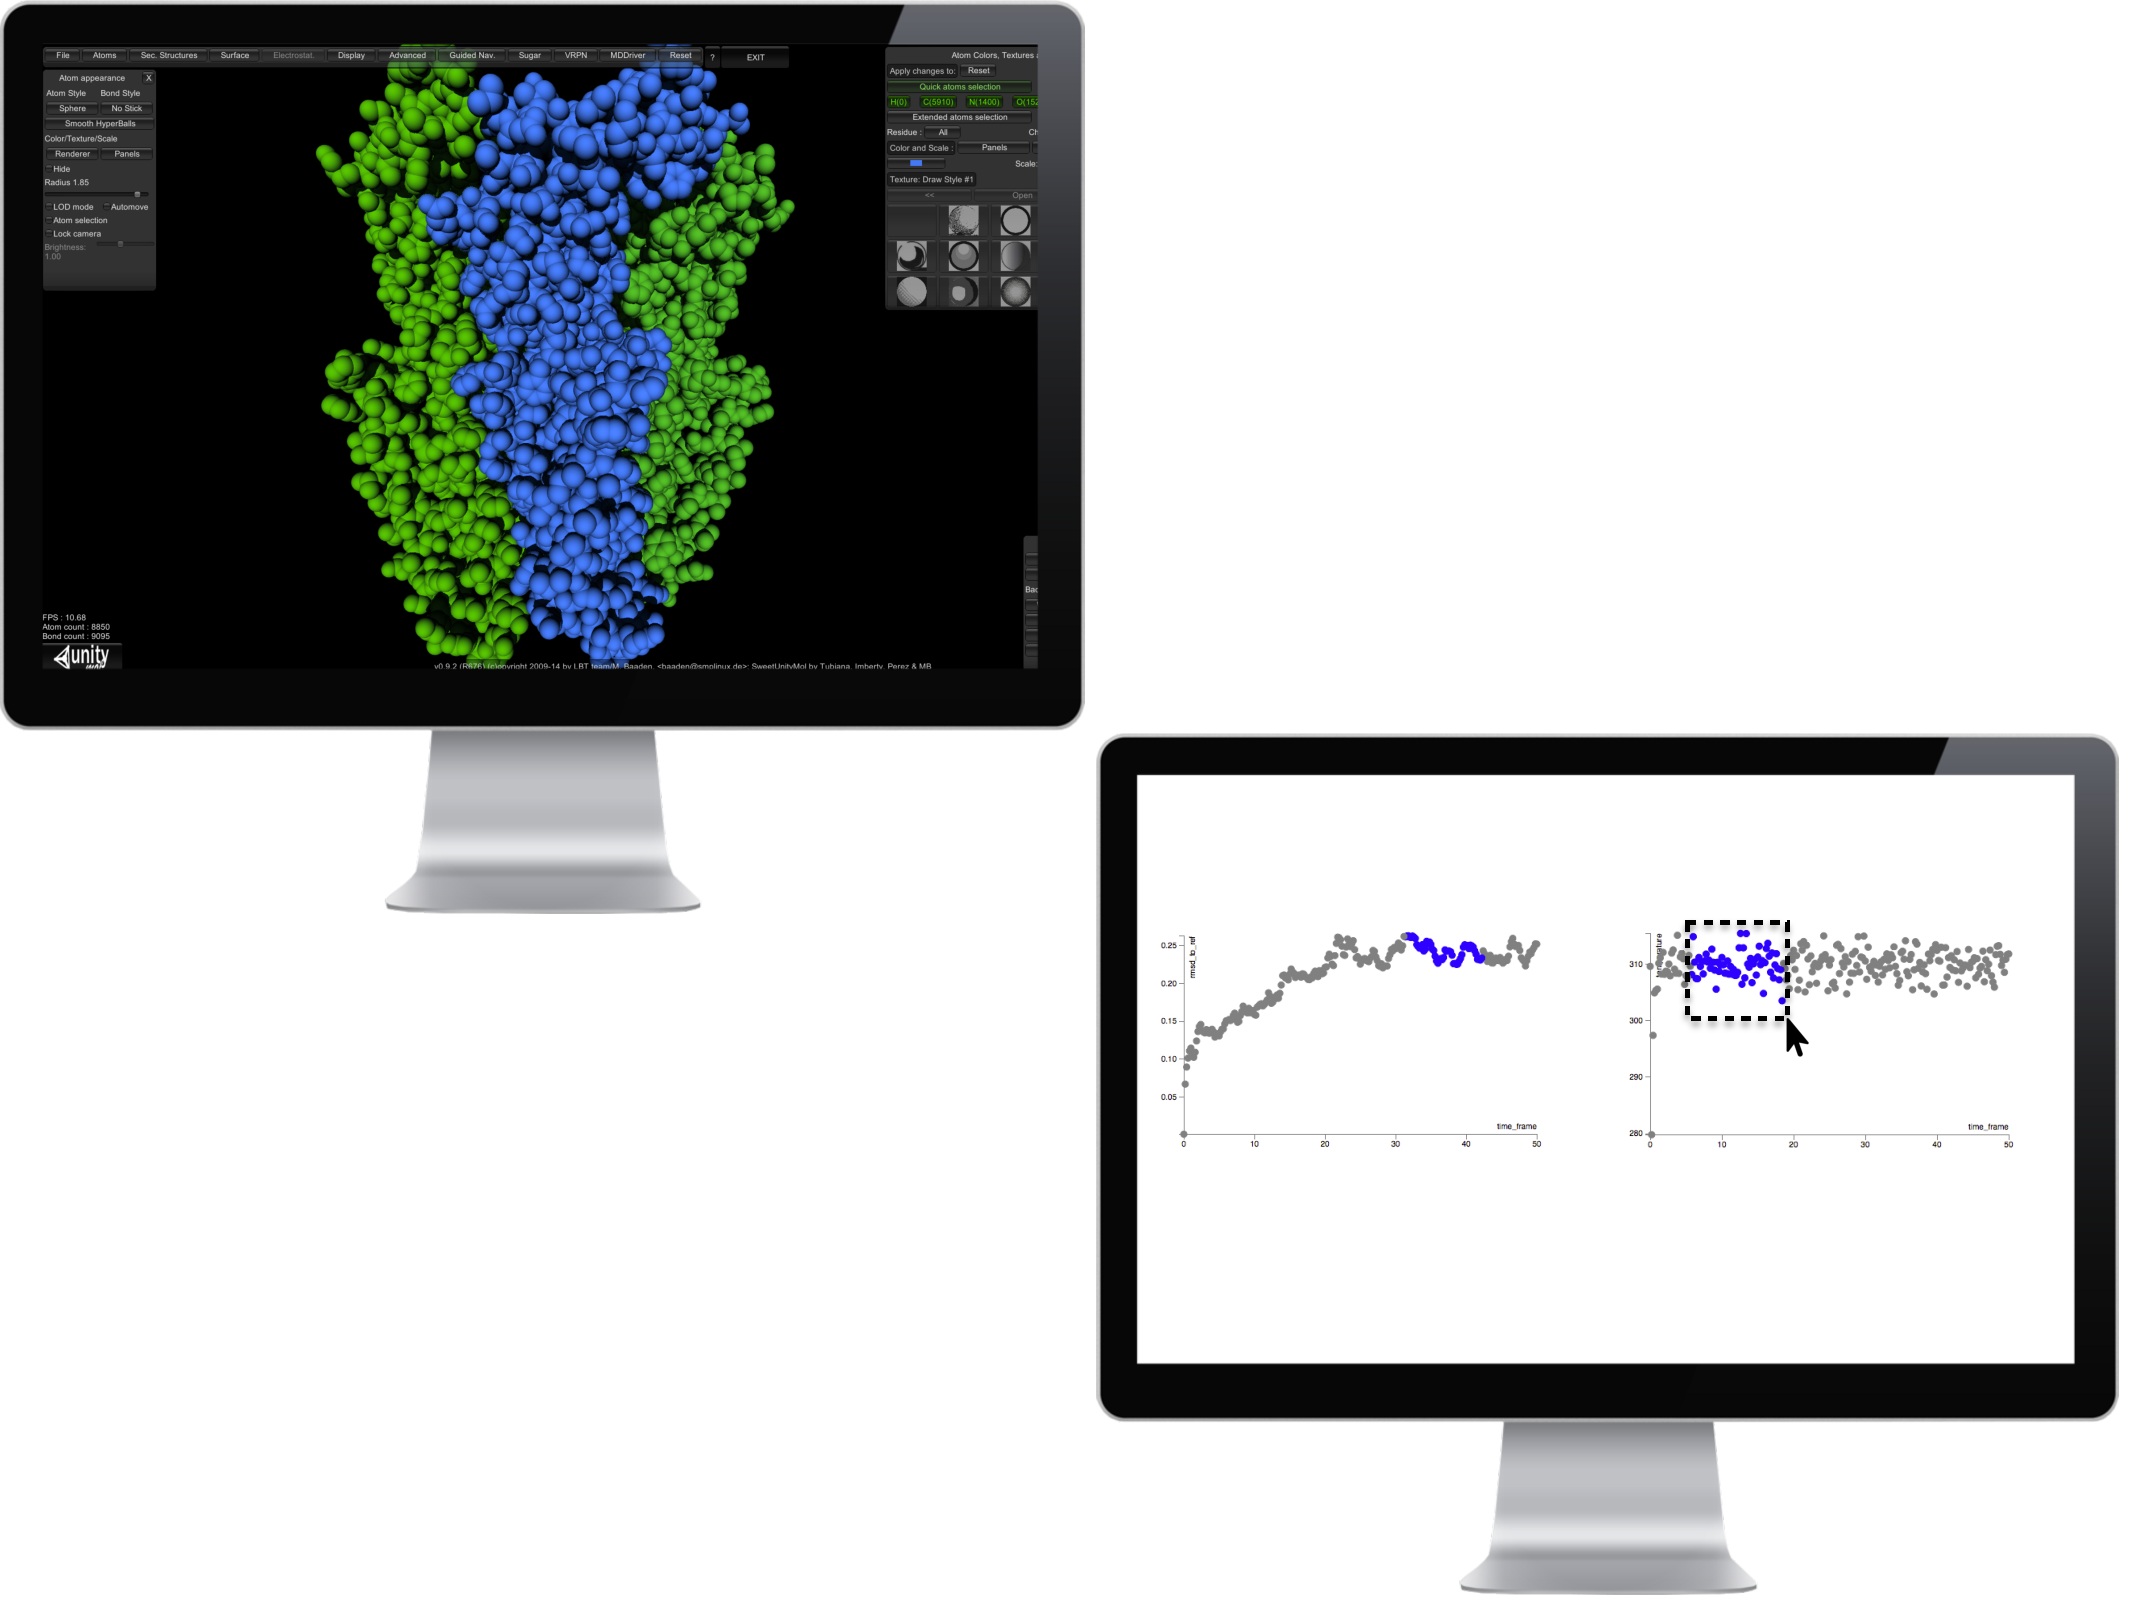
\includegraphics[width=.75\linewidth]{./figures/ch4/ch4_visu2d_visu3d_link.pdf}}
    \caption{\it Illustration du lien entre des diagrammes de dispersion présentant deux résultats d'analyses et un visualiseur 3d. Une sélection d'individus dans les diagrammes entraîne une coloration et une mise en avant de la représentation 3d de ces mêmes individus.}
  \label{Fig:bilateral_selection}
  \hspace{0.3cm}
\end{figure}

\subsection{Applications en RV}



% Intro sémantique / données liées
\subsection{Représentation des connaissances}

La notion de représentation des concepts et des liens entre ces concepts est connue des sciences informatiques et plusieurs formalismes en découlent. La mise en place d'ontologies afin de standardiser les connaissances dans des domaines de recherche scientifique a connu un développement spontané et important à partir de la fin des années 90 \cite{schulze-kremer_ontologies_2002, baker_ontology_1999}. 
Une ontologie est \textit{l'ensemble structuré des termes et concepts représentant le sens d'un champ d'informations, que ce soit par les métadonnées d'un espace de noms, ou les éléments d'un domaine de connaissances.}\footnote{\url{https://fr.wikipedia.org/wiki/Ontologie_\%28informatique\%29}}. Une ontologie se définit comme un vocabulaire cherchant à classer des concepts et définir des relations entre ces concepts pour un domaine spécifique. Ce classement hiérarchique se doit d'être interprétable à la fois par les machines et les humains. Tout d'abord afin d'être intégrer dans des processus informatiques et ensuite afin de servir de modèle aux scientifiques pour l'élaboration de bases de données résultantes d'ontologies.

\subsubsection{Choix du formalisme}

Afin de correctement manipuler les connaissances et les données sous-jacentes, il convient de choisir un formalisme adapté à notre objectif. Le formalisme utilisé pour représenter des connaissances dépend à la fois du domaine d'application (ici la biologie structurale), des opérations à mettre en oeuvre sur ces connaissances (lier les faits entre-eux, extraire de nouvelles connaissances, obtenir des descripteurs pertinents pour l'aide à la décision) et des processus d'implémentation qui seront utilisés (nous désirons utiliser ce formalisme au sein d'une suite logicielle multi-composants performante). Au sein des formalismes, il est possible de distinguer deux classes d'approches, les approches non logiques et les approches logiques.

Les approches non logiques regroupent des logiques descriptives comme les \textit{réseaux sémantiques} et les \textit{Graphes Conceptuels}.
Les approches logiques regroupent les \textit{logiques classiques} comme la logique propositionnelle, de 1er ordre ou de 2e ordre ainsi que les \textit{logiques de description}.

\paragraph{Réseaux sémantiques}

Les réseaux sémantiques sont destinés à la modélisation hiérarchique de connaissances sous forme de graphes marqués. Un réseau sémantique contient des concepts, représenté par des noeuds et des relations, représentés par des liens (ou arcs) étiquetés entre chaque noeud. Ils ont été dans les années 60 par Quillian et Collins \cite{collins1969retrieval} comme base pour la représentation taxonomique. Ils se caractérisent par des relations binaires entre les concepts de type \textit{est-un}, \textit{a} ou \textit{type-de}.

\paragraph{Graphes Conceptuels}

Les graphes conceptuels, introduits par Sowa en 1984 \cite{sowa1983conceptual}, tiennent leur origine des réseaux sémantiques \cite{lehmann1992semantic} et sont un moyen de formaliser les connaissances \cite{chein2008graph}. Ce modèle est mathématiquement fondé sur la logique et la théorie des graphes. Cependant, pour raisonner à l'aide de GC, deux approches peuvent être distinguées : (1) considérer les GC comme une interface graphique pour la logique et donc raisonner à l’aide de la logique et (2) considérer les GC comme un modèle de représentation à part entière disposant de ses propres mécanismes de raisonnement fondés sur la théorie des graphes. Dans ce modèle, les concepts et les relations sont des noeuds reliés par des arcs orientés comme illustré dans la figure X. Les connaissances sont donc représentées par des graphes étiquetés dont les mécanismes de raisonnement se basent sur des opérations de graphes et en particulier sur l'\textit{homomorphisme} de graphes (anciennement \textit{projection}).
Un des inconvénients des graphes conceptuels réside dans leur faible utilisation au sein de la communauté scientifique. Peu de librairies ou applications supportant la notion de graphes conceptuels et la théorie des graphes qu'elle utilise existent. Leur implémentation au sein de suites logicielles en est donc partiellement difficile quand d'autres formalismes proches comportent une intégration plus importante au sein des langages de programmation les plus utilisés. De plus, ils sont exclusivement descriptifs et n'ont que peu d'extensions visées à leur adjoindre une sémantique basée sur la logique afin de pouvoir en extraire des connaissances supplémentaires.

\paragraph{Logique classique}

Les logiques de 1er ordre, 2e ordre et propositionnelles sont 3 propositions de logiques dites "classiques" présentation une première formalisation du langage et du raisonnement mathématique. Cette logique est caractérisée par des postulats qui la fondent:

\begin{itemize}
	\item Le \textit{tiers exclu} énonce que pour toute proposition mathématique considérée, elle même ou sa négation est vraie.
	\item Le \textit{raisonnement par l'absurde} qui veut prouver qu'une proposition est vraie non pas en la démontrant mais on démontrant que la proposition contraire est absurde.
	\item La \textit{contraposition} qui consiste à dire qu'une implication de type "A implique B" permet de dire que "si non-B alors non-A". B est donc une condition nécessaire de A.
	\item L'\textit{implication matérielle} ou le "seulement si" ou "si ..., alors ..." qui en logique classique se caractérise par la volonté de donner une valeur de vérité à toute proposition. Par exemple "s'il pleut, alors mon gazon est mouillé." Cette proposition ne permet pas de dire, "si mon gazon est mouillé, alors il pleut".
	\item Les \textit{lois de Morgan} qui sont des identités entre propositions logiques énonçant que "non(A et B) est (non A) ou (non B)" et "non(A ou B) est (non A) et (non B)".
\end{itemize}

Parmi les logiques classiques, la logique du 1er ordre (ou calcul des prédicats) introduit les symboles mathématiques permettant de formuler des modèles de relations au sein d'ensembles mathématiques. On retrouve dans ces symboles: Les variables, les prédicats (ou relations), les connecteurs logiques (et, ou, etc.) et deux quantificateurs universel \forall ("Quel que soit", "Pour tout") et existentiel \exists ("il existe au moins un ... tel que"). Les formules logiques déduites des énoncés de calculs de prédicats ont pour but de s'appliquer à n'importe quel modèle où l'on retrouve des variables, des fonctions et des prédicats représentant respectivement les éléments de l'ensemble, les fonctions de l'ensemble et les parties (ou sous-ensembles) de l'ensemble.


\paragraph{Logique de description}

Ces logiques se rapportent à la fois à la description des concepts décrivant un domaine et à la fois à la sémantique basée sur la logique. Cette logique est un apport par rapport aux réseaux sémantiques qui ne possèdent pas de sémantique basée sur la logique et sont donc exclusivement descriptives. C'est une famille de langage permettant d'une part la description des connaissances d'un domaine de façon structurée et formelle et d'autre part elles possèdent une sémantique formelle définie en logique du 1er ordre. Elles sont utilisées pour de nombreuses applications dont le web sémantique et la bio-informatique et particulièrement les ontologies associées. 
Similairement aux logiques classiques, les logiques de description utilisent les notions de \textit{concept}, \textit{rôle} et \textit{individu} \cite{baader2003description}. Les \textit{concepts} désignent les sous-ensemble d'élément dans un univers étudié, les \textit{rôles} correspondent aux liens entre les éléments et enfin les \textit{individus} sont les éléments de l'univers.


\subsubsection{Applications}

La génomique fut le domaine biologique qui a vu le premier la nécessité d'utiliser des ontologies afin d'uniformiser la quantité de données toujours plus importante générée et intégrée dans des bases de données hétérogènes à travers le monde \cite{schuurman_ontologies_2008}.
En génomique et protéomique, de nombreuses études s'appuient sur l'aide directe ou indirecte de \textit{Gene Ontology} \cite{ashburner_gene_2000}, une "bio-ontologie" qui a résulté de la prolifération de jeux de données à l'échelle génomique et la mise en place de protocoles pour l'échange et le partage de données sur le web. Elle fut le fruit de la nécessité, lors de l'explosion du nombre de données générées, de mettre en place un vocabulaire standard que les scientifiques pourraient utiliser afin de classifier et renseigner leurs données. GO n'est pas totalement considéré comme une ontologie selon la définition informatique stricte du terme car il ne possède pas de règles d'inférence complexes, ne se basant pas sur une description logique de ses concepts et sur des inférences simples de type \textit{est-un} ou \textit{est-une-partie-de}. Il est davantage mis en avant comme un vocabulaire standardisé des concepts mis en jeu dans les recherches afin de mettre en place un espace commun de termes précis et définis, possédant une hiérarchie établie. Il permet donc de mettre en relation des bases de données hétérogènes respectant ses codes ontologiques et donc d'effectuer des opérations de requêtes croisées ou de comparaison. Progressivement de nombreuses autres "bio-ontologies" sont apparues dans la lignée de GO et plusieurs d'entre-elles ont permis de mettre en avant, via le simple mécanisme d'inférence et de mise en relations des données hétérogènes, de nouvelles avancées en biologie \cite{yoshikawa_drug_2004, stenzhorn_biotop_2008, smith_obo_2007}.

Enfin, plusieurs programmes de visualisation analytique se sont appuyés sur la mise en place d'une sémantique décrivant les concepts mis en jeu \cite{rysavy_dive:_2014}. Cette représentation participe à la formalisation des concepts analysés et instaure un premier lien entre les différents modules d'un programme cherchant à partager visualisation et analyses au sein d'un même espace de travail. DIVE constitue un premier exemple de programme possédant un procédé logiciel incluant la mise en place automatique d'une ontologie afin de classer les données et de refléter le modèle de données utilisé par les librairies utilisées durant la session de visualisation et d'analyse. Le parseur mis en place dans DIVE traduit une architecture .NET \footnote{\url{https://microsoft.com/net}} en une structure de donnée hiérarchique. Chaque valeur de donnée est partagée entre l'architecture .NET et les représentations correspondantes dans DIVE permettant une modification/évolution dynamique de celle-ci pendant l’exécution du programme. Cette solution permet également de mettre en place des méthodes de requêtes sur les valeurs ou les relations entre les objets représentés et donc de mettre en avant de nouvelles informations sur les sets de données étudiés. DIVE se rapproche par plusieurs aspects de nos travaux, cependant, plusieurs points distinguent nos deux approches. Tout d'abord, afin de permettre un pré-traitement et une harmonisation des données manipulées, notre ontologie est pré-définie, imposant un contexte de travail précis et fixe. Cela favorise la mise en place de nouveaux modules car l'utilisateur sait quels concepts et propriétés sont mis en jeu dans notre processus. Comme nous l'avons fait remarquer, notre ontologie garde une certaine souplesse puisqu'il est aisément possible de l'étendre à de nouveaux concepts et propriétés suivant les besoin. Il est cependant nécessaire de garder le vocabulaire de base de l'ontologie pour pouvoir profiter de toutes les fonctions en découlant. Notre ontologie est spécifique à notre domaine d'étude, qui est la biologie structurale et plus particulièrement la visualisation et l'analyse de données de modèles de molécules dynamiques ou non. DIVE est capable de fournir une architecture plus globale puisque s'adaptant à chaque set de données mis en jeu. L'inférence propre aux ontologies est également limitée dans DIVE puisqu'elle se limite à une notion d'héritage propre au modèle OO de certains langages de programmation.


\subsection{Web sémantique et formalismes à base de graphes}

Le Web sémantique est un mouvement collaboratif mené par le \textit{World Wide Web Consortium} visant à développer des méthodes communes pour l'échange de données sur le Web. Le but du Web sémantique est de structurer et lier les connaissances présentes sur internet afin d'en faciliter le traitement et la recherche à travers le monde. Selon la définition même du W3C, \textit{le Web sémantique fournit un modèle qui permet aux données d'être partagées et réutilisées entre plusieurs applications, entreprises et groupes d'utilisateurs.} Le concept de Web sémantique n'est pas un modèle universellement adopté et, pour le moment, il se retrouve seulement dans plusieurs initiatives indépendantes attachées aux domaines de l'industrie, de la biologie et des sciences humaines. Plusieurs chercheurs ont travaillé à son utilisation et les conséquences d'un passage de l'ensemble des acteurs du web à un tel concept \cite{feigenbaum_semantic_2007}. Nous pouvons citer comme initiatives notables DBpedia, un effort pour publier les données extraites de wikipedia sous format RDF et interrogeables via SPARQL que nous décrivons ci-après \cite{auer2007dbpedia} ou le projet Data.bnf.fr\footnote{\url{http://data.bnf.fr}} qui intègre des données provenant de formats divers (Itermarc\footnote{\url{http://www.bnf.fr/fr/professionnels/f_intermarc/s.format_intermarc_biblio.html}}, XML-EAD et Dublin Core \cite{weibel1998dublin} pour la bibliothèque numérique), les regroupant et les formalisant par des traitements automatiques et les publiant dans divers standards du Web sémantique basés sur le RDF \textit{Resource Description Framework} (RDF-XML, RDF-N3 et RDF-NT, voir section \ref{rdf_model}.
Le Web sémantique se base sur un formalisme grandement inspiré des logiques de description. Le modèle de graphe associé au web sémantique est le RDF \cite{klyne2006resource}. Il est structuré par le RDFS (RDF Schema) \cite{brickley2004rdf} qui décrit les vocabulaires (ontologies) sur lesquelles des ressources RDF se basent à la manière d'une DTD (Document Type Definition) pour le XML (eXtensible Markup Language) qui permet de mettre en place une hiérarchie au niveau des balises utilisée dans un document XML. 
L'ensemble des caractéristiques principales du RDFS sont repris dans un langage ontologique plus expressif appelé OWL \cite{mcguinness2004owl}. OWL fonctionne de la même manière que RDFS en étendant certaines logiques sémantiques pour le RDF. La structuration des ressources RDF avec RDFS et OWL permet l'interrogation de ces ressources par le langage de requête SPARQL (SPARQL Protocol and RDF Query Language) \cite{prud2008sparql}. RDF, RDFS, OWL et SPARQL sont tous les 4 des recommandations du W3C pour le Web sémantique et ils disposent d'une intégration de plus en plus élargie au sein des technologies et contenus web destinés au partage de connaissances et à leur traitement.

\subsubsection{Modèle RDF} \label{rdf_model}

Le langage RDF est le langage de base du Web Sémantique qui l'utilise afin de mettre en place un réseau de données partagées et libres. C'est un modèle de graphe destiné à décrire de façon formelle des ressources et leurs métadonnées associées, de façon à permettre leur traitement automatique.

Le modèle RDF se base sur une représentation des connaissances à partir de triplets. Le triplet est la plus petite division de connaissances en RDF et toute description de données est un ensemble de triplets comprenant:

\textit{(sujet, prédicat, objet)}

Le \textit{sujet} représente la ressource que nous cherchons à décrire. Le \textit{prédicat} représente une propriété pouvant être associée à la ressource. L'\textit{objet} peut représenter soit une ressource, soit une donnée, cela correspond à la valeur de la propriété.
Chaque ressource est identifiée par une URI (Uniform Ressource Identifier) alors qu'une donnée est anonyme puisque pouvant être dupliquée (valeur numérique, chaîne de caractère, etc.). Un exemple de triplet pourrait être:

\textit{(http://mon-ontologie.fr/\#Pierre, http://mon-ontologie.fr/\#âge, xsd:int\#26)}

Les ressources de ce triplet (\textit{sujet} et \textit{prédicat}) sont décris par leur URI qui est constitué d'une partie fixe (\textit{http://mon-ontologie.fr/\#}) identifiant le moyen de localiser la ressource et une partie variable (\textit{Pierre} et \textit{âge}) correspondant au nom de la ressource identifiée. Les URI les plus connues et utilisées sont les URL permettant d'accéder à des ressources internet mais les numéros ISBN référençant les livres sont également des URI.
Dans des termes propres aux bases de données relationnelles SQL, RDF peut être considéré comme une table composée de 3 colonnes, sujet, prédicat, objet. A la différence de SQL cependant, la colonne objet est hétérogène et le type de donnée par cellule est sous-entendue (ou spécifié dans l'ontologie, voir \ref{rdfs}) par la valeur du prédicat.

De la même manière que les graphes conceptuels, le document RDF décrivant un ensemble de données peut être représenté par un multigraphe orienté étiqueté. Chaque triplet est représenté par un arc orienté dont les extrémités sont le sujet et l'objet et le label de l'arc correspond au prédicat.

Le modèle de représentation RDF s'appuie sur un formalisme précis et standardisé qui permet l'uniformisation des données représentées et la mise en place de lien entre ces données. Ce formalisme n'est qu'une méthode de représentation et ne constitue pas une logique de raisonnement qui permettrait d'extraire des connaissances de ces données. C'est dans ce but qu'a été créé RDFS et OWL, des langages formels servant à décrire des ontologies. A la différence des données RDF qui sont de l'ordre du \textit{factuel}, une ontologie permet de décrire les concepts et les relations entre ces concepts et constitue la partie \textit{structurelle} du Web sémantique.
OWL et RDFS reprennent les critères standards des ontologies existantes et qui est le support de nombreuses ontologies recensées dans le portails officiels de bio-ontologies largement utilisées dans la communauté scientifique \cite{smith_obo_2007}.

\subsubsection{RDF Schema} \label{rdfs}

RDFS fut la première extension permettant d'ajouter une couche sémantique au modèle de ressource RDF. Il définit les notions de classes, sous-classes, propriétés et sous-propriétés desquelles dépendront les ressources RDF identifiées. C'est donc un ensemble de concepts haut-niveau définissant les différents individus d'un domaine et permettant leur hiérarchisation. 
Par exemple, RDF permet de décrire qu'une <Lysine> \textit{a une charge} <positive> grâce aux individus <Lysine> et <positive>, respectivement sujet et objet, et au prédicat \textit{a une charge}. RDFS permet d'ajouter les concepts décrivant les individus comme <Acide-aminé>, <Charge>, <Hydrophobicité>, <Molécule>, etc. et de préciser des relations entre ces groupes de façon à pouvoir émettre des déductions simples. Par extension de l'exemple précédent, si l'on ajoute que tout <Acide-Aminé> est une <Molécule> qui revient à dire en RDFS, <Acide-aminé> \textit{sous-classe de} <Molécule>, et <Lysine> \textit{instance de} <Acide-aminé>. Cela nous permet d'ajouter un niveau d'information induite des deux affirmations précédente qui serait: <Lysine> \textit{instance de} <Molécule>. Cette déduction se fait grâce au système d'implication introduit par RDFS et permettant de déduire des informations complémentaires à partir d'un minimum de données.

RDFS introduit également la notion de domaine de définition (\textit{rdfs:domain}) et d'ensemble d'arrivée (\textit{rdfs:range}) pour les propriétés. Le domaine de définition correspond à la classe des sujets liés à une propriété alors que l'ensemble d'arrivée correspond à la classe ou au type de données des valeurs de la propriété. Il est par exemple possible de préciser que la propriété <identifiant> doit avoir comme domaine de définition seulement des individus de classe <Objets> et comme ensemble de définition des valeurs de type <xsd:integer>.
Le système d'implication de RDFS fonctionne également avec les notions de domaine d'application et d'ensemble de définition. De ce fait, ces 3 affirmations:

<Alanine> \textit{est-un} <Acide-aminé>,
<Protéine> \textit{contient} <Lysine>,
<contient> \textit{rdfs:range} <Acide-aminé> 

permettent d'induire l'affirmation suivante:

<Lysine> \textit{est-un} <Acide-aminé>


\subsubsection{OWL}

OWL est donc un standard informatique visant également à jouer le rôle de grammaire pour le langage RDF en complément du RDFS à qui il reprend ses bases. Le langage OWL se base sur des éléments des logiques de description et constitue un standard informatique permettant de vérifier que les données soient cohérentes, de déduire de nouvelles connaissances de ces données ou d'en extraire certaines informations.
Plus expressif que RDFS, OWL permet d'adjoindre à la définition des relations entre objets par des assertions fournie par RDFS, des propriétés reliant les classes à travers des relations de symétrie, d'équivalences, de cardinalité, etc. entre les classes. 
Il est donc possible de mettre en place des associations de classes et de propriétés plus complexes et basée sur une fondation logique  

Si l'on étend l'exemple précédent avec les notions apportées par OWL au sein des triplets suivants:

<est-composé-de> \textit{est} <owl:TransitiveProperty>,
<Protéine> <est-composé-de> <Acide-aminé>,
<Acide-aminé> <est-composé-de> <Atome>

nous pouvons donc en déduire, grâce au caractère transitif de la propriété <est-composé-de>, que:

<Protéine> <est-composé-de> <Atome>

De la même manière, il est possible de définir des propriétés comme symétriques, asymétriques, inverses, réflexives, etc.\footnote{\url{http://www.w3.org/2007/OWL/wiki/Quick_Reference_Guide}}
OWL est composé de 3 sous-langages classés du moins expressif au plus expressif: OWL-Lite, OWL-DL et OWL-Full. Parmi ces sous-langages, seul OWL-Lite est implémenté sous forme d'algorithmes décidables dans la majorité des moteurs d'inférence utilisé lors de l'interrogation de bases de données RDF possédant une ontologie OWL associée. La simplicité d'OWL-Lite lui permet une complexité réduite et donc un temps de calcul également réduit lors de son utilisation. Il regroupe les principales relations et descriptions de classe amenée par OWL et permet ainsi une mise en place de logiques descriptives suffisamment évoluées pour permettre l'extraction de nouvelles connaissances à partir de données simples.

\subsection{SPARQL}

Nous venons d'évoquer la possibilité d'utiliser un moteur d'inférence afin d'extraire des données d'une base de données RDF. Cette extraction peut se faire via l'utilisation d'un protocole et langage de requête appelé SPARQL. Ce langage permet à la fois de récupérer des données stockées sous format RDF dans une base de données mais également de les éditer, d'en ajouter ou bien d'en supprimer. L'accès aux bases de données se fait grâce à une interface d'accès (en anglais \textit{endpoint}) géré par un service capable de recevoir des requêtes SPARQL et de renvoyer des résultats sous différents formats.
A la différence du SQL, SPARQL se base essentiellement sur le format en triplets des bases de données RDF et la majorité de ses requêtes repose sur la mise en place d'un schéma de correspondance entre triplets sujet/prédicat/objet. Il n'y a pas de contraintes de typage pour la colonne objet qui est habituellement implicite ou définie par l'ontologie. Dans le même esprit, l'ontologie est directement intégrée dans les résultats de requêtes et le schéma de données n'a donc pas besoin d'être appliqué de façon séparée. SPARQL fournit également plusieurs opérations sur les résultats comme SORT, JOIN, DISTINCT, qui permettent un traitement direct des résultats afin de les classer ou filtrer suivant les besoins...\footnote{\url{http://www.cambridgesemantics.com/semantic-university/sparql-vs-sql-intro}} Certains mots-clés de SQL ont été conservé tels que SELECT, FROM, WHERE, etc.

De nombreuses librairies permettent d'utiliser des points d'accès SPARQL afin d'y présenter des requêtes et d'en récupérer leurs résultats. Cette implémentation présente dans de nombreux langages de programmation assure une certaine généricité du travail d'interfaçage nécessaire dans une suite logicielle multi-composants.

\subsection{Visualisation analytique interactive pour les données scientifiques}

\subsubsection{Bio-ontologies}

\cite{schulze-kremer_ontologies_2002}

\subsubsection{Web sémantique et formalismes à base de graphes}

Sesame [55] est une architecture générique pour le stockage persistant de RDF(S) dans une base de données et l'interrogation de ce RDF(S) avec le langage RQL. RQL [56] est un langage de requête RDF défini par le moyen d'un ensemble de requêtes fondamentales, un ensemble de filtres de base et un moyen de construire de nouvelles requêtes par une composition fonctionnelle et des itérateurs. Lors de l'analyse d’une requête RQL, Sesame construit une requête optimisée évaluée au moyen d'une série d'appels à la couche de stockage et d’inférence de Sesame.

Par comparaison RDQL [56] permet l'interrogation de données RDF au niveau de la structure, tandis que Sesame permet l’interrogation au niveau sémantique. En ce sens notre objectif est beaucoup plus proche de Sesame. Toutefois Sesame ne considère pas la sémantique des XSD datatypes, ni ne permet d’avoir des règles d'inférence exploitant les ontologies.

Jena [57] est l’un des moteurs actuels les plus complets et propose une persistance en mémoire ou en base de données. Il implante RDF, RDFS et OWL ainsi que les requêtes SPARQL et propose un moteur en chaînage avant (RETE), arrière (programmation logique) et hybride. Ce moteur est utilisé pour implanter la sémantique de RDFS et OWL. Le modèle de Jena repose sur une structure prédéfinie de bases de données.

Triple [58] est un langage de requêtes pour divers modèles de données du web sémantique. Le noyau Triple est un langage de requête RDF fondé sur la logique de Horn étendue par des fonctionnalités syntaxiques pour intégrer des primitives RDF comme les espaces de nommage, les ressources et les réifications. Ce langage peut être compilé en logique de Horn et exécuté par des moteurs Prolog. Triple n'est pas limité à l'interrogation de données RDF. Il dispose d'une architecture en couche lui permettant d'interroger d’autres modèles de données avec différents types de sémantique (ex : RDFS et DAML + OIL) et en ce sens il rejoint notre certitude qu’il faut abstraire les structures et algorithmes des différents langages que nous manipulons. Le noyau de Triple est étendu par des règles pour l’axiomatisation de la sémantique de RDFS ; elles peuvent être utilisées avec un moteur d'inférence pour dériver des connaissances supplémentaires à partir d'un schéma RDFS.

DAMLJessKB [59] et son successeur OWLJessKB ainsi que le cœur du eWallet [13] sont des outils de raisonnement pour DAML [60] ou OWL Lite. Ils ont tous les trois intégré JESS [61] un moteur de règles de production qu’ils appliquent à la sémantique de RDF, RDFS, DAML, XSD (XML Schema Datatypes [62]) et OWL Lite. Ils implantent une traduction des triplets RDF vers des faits du langage CLIPS de Jess et utilisent des règles de production pour décrire la sémantique des langages traduits. A l'aide de Jess, ces systèmes peuvent effectuer des raisonnements sur les classes et les instances.

OntoBroker [63] et son successeur On2broker sont des pionniers des systèmes à base d'ontologies basés sur les Frame Logics. OntoBroker gère des métadonnées intégrées dans des documents HTML avec des balises tout comme On2Brocker gère des annotations RDF. Dans les deux systèmes, les ontologies et les requêtes sont exprimées en langage frame logics qui permet la représentation d'une hiérarchie de types de concepts, d'une hiérarchie de types de relations et de règles. Le moteur de requête traduit ces représentations en Logique de Horn pour répondre à une requête.

OntoBroker, On2Broker, DAMLJessKB, OWLJessKB et partagent avec notre initiative le même principe général et les expressivités de leurs langages de représentation à base d’ontologie sont comparables. Toutefois, ces systèmes sont dédiés à des capacités générales de raisonnement sans exploiter les structures de graphes par exemple pour optimiser des opérations spécifiques à la recherche d'informations. Leurs langages de requêtes sont proches des logiques sur lesquelles ils se basent et restent dans leurs limites.

WebKB [64] [65] est un pionnier des serveurs web d'ontologies et des robots web basés sur les graphes conceptuels. Sur la base de sa simplicité et de l'exhaustivité de sa représentation, ses auteurs rejettent l'utilisation directe des langages basés sur XML. WebKB interprète et traduit automatiquement en graphes conceptuels des déclarations exprimées dans une notation linéaire des graphes et intégrées à des documents web. WebKB fournit des commandes de requête pour interroger les propriétés lexicales ou structurelles des documents HTML ou afficher des spécialisations ou généralisations d'un concept, d'une relation ou d'un graphe.

OntoSeek [66] est un autre système conçu pour la recherche d’information basée sur le contenu de pages jaunes et de catalogues de produits en ligne. Il combine les graphes conceptuels et des ontologies du domaine correspondant. Il met l'accent sur les contraintes lexicale et sémantique dans le codage des ressources en graphes conceptuels et la construction de requêtes. Requêtes et annotations des ressources sont des graphes conceptuels lexicaux entre lesquels on cherche des homomorphismes.

WebKB, OntoSeek et la plate-forme que nous spécifierons en section 3.3.4 partagent le même type de représentation à base de graphes, par conséquent, le même principe d’homomorphisme correspondant à une requête sur les graphes d'annotation en prenant en compte la subsomption des types de concepts et des types de relations. Mais ni WebKB ni OntoSeek n’intègre RDF(S) ou les règles dans leur représentation à base d’ontologie.

Avec la standardisation de OWL DL, les moteurs à base de logiques de descriptions ont pris une importance particulière. Citons : Fact et son successeur Fact ++ [67], KAON2 [68] (une branche de KAON qui lui est resté focalisé sur RDFS), Racer [69], Pellet [70]. Ces moteurs offrent des opérations classiques en logiques de descriptions : identification, classification, validation. L’interrogation se limite en général à des requêtes conjonctives et les mécanismes d’interrogation ne sont pas prévus pour exploiter la structure des graphes ni accepter des graphes de grande taille.

En conclusion, aucune des contributions citées ci-dessus ne cherche à mettre en place un modèle pivot et une plate-forme ouverte et open-source pour implanter efficacement les aspects des représentations relevant des graphes. Elles sont toutes liées à un langage particulier (le plus souvent une logique) et/ou à une application particulière.

En ce qui concerne les outils permettant de raisonner avec des graphes conceptuels, les deux principaux outils sont : CoGITaNt [71] développé conjointement par le LIRMM et le LERIA, plate-forme dédiée à la mise en œuvre de mécanismes de raisonnement sur les graphes conceptuels spécifiquement ; et Amine (développé par l'INSEA au Maroc), plate-forme dédiée au développement de systèmes intelligents, qui repose sur une combinaison de Prolog et de graphes conceptuels. Citons également Prolog+CG basé sur un précurseur d'Amine, à usage éducatif.

Corese [72] [73] [5] [74] est un moteur de recherche sémantique basé sur les graphes conceptuels. Il implante RDF/S et SPARQL et il est développé dans l’équipe Acacia puis Edelweiss. Plus précisément, il implante la sémantique de RDF, RDFS, ainsi que les datatypes, les propriétés transitives, symétriques et inverses de OWL Lite.

Comme le montre la Figure 31, CORESE combine les avantages d'utiliser le langage RDF(S)/XML pour exprimer et échanger des méta-données, et les mécanismes de requête et d'inférence disponibles pour le formalisme des Graphes Conceptuels.

\section{Problématique}

\subsection{Limites actuelles en biologie structurale}

L'analyse de structures moléculaires est cruciale pour la compréhension de la fonction métaboliques des complexes moléculaires. Nous avons mis en avant les différentes étapes et les moyens disponibles pour récolter un maximum d'informations quant à la structuration d'une biomolécule. La précision des outils expérimentaux et computationnels ainsi que leur efficacité a entraîné la mise en place d'un flux de données en biologie structurale dont la taille et la vitesse dépassent désormais les capacités d'analyses des experts et des outils qu'ils utilisent. 

La complexité des données est par exemple en constante progression. La taille même des structures désormais observées et étudiées augmente puisqu'il est maintenant possible de simuler des systèmes de plusieurs millions d'atomes pendant des durées biologiques pertinentes, de l'ordre de la nanoseconde, permettant d'observer des phénomènes structuraux précis. La visualisation de capsides virales, de ribosomes ou de complexes membranaires entiers demande des performances importantes de la part des logiciels de visualisation. Ces derniers ont donc du s'adapter et évoluer pour répondre à ces nouveaux défis visuels. Le calcul sur processeur graphique a permis de franchir une grande étape en terme de performance et plusieurs algorithmes de rendus graphiques largement utilisés au sein des logiciels de visualisation en ont profité \cite{chavent_gpu-powered_2011}. En parallèle, de nouvelles techniques de rendus graphiques, inspirées pour certaines du monde du jeu vidéo, ont vu le jour afin de rapprocher les représentations de molécules de représentations d'objets réels, réduisant ainsi la perception complètement artificielle des objets observés \cite{lv_game_2013}. Les progrès effectués ont également permis de rendre la visualisation moléculaire plus interactive puisque plus réactive et plus performante, accordant ainsi aux utilisateurs davantage de possibilités quant à leurs options de rendus et dépassant ainsi la simple image statique et pré-calculée de structure 3d.

Cependant, ces récentes avancées ne sont pas suffisantes pour rapporter la complexité des complexes moléculaires les plus importants. La limitation n'est pas dans l'efficacité du rendu mais dans la façon de présenter les structures 3d d'intérêt. Il est nécessaire de passer un palier dans les habitudes d'observation de structures moléculaires en prenant en compte leur nature 3d et en utilisant les progrès effectués en Réalité Virtuelle afin d'immerger les utilisateurs au sein de leurs structures afin qu'ils en extraits toutes les informations possibles. De la même manière, la possibilité de créer un monde virtuel entier ouvre d'importantes portes pour l'association d'informations, d'analyses et d'interactions avec ces structures afin de les enrichir. 

Or nous avons souligné auparavant les caractéristiques de la RV et ce qu'elle impliquait, à savoir davantage qu'un simple rendu stéréoscopique, la mise en place d'interactions adaptées et pertinentes pour la tâche experte prévue.
Parmi les problématiques soulevées par la RV, nous avons déjà évoqué la navigation au sein des mondes virtuels comme l'un des obstacles cruciaux à franchir pour assurer une expérience optimale aux utilisateurs. En effet, la notion de monde virtuel implique la possibilité pour l'utilisateur d'évoluer au sein d'un environnement étendu de la même manière qu'il évoluerait dans la vie réelle. Or, si cette navigation virtuelle peut être approchée par le biais de la navigation réelle dans le cas d'environnements virtuels écologiques, à savoir où le contenu virtuel proposé n'est qu'une copie artificielle d'éléments réels, la question est toute autre lorsque la scène observée n'est plus écologiques et impliquent des éléments abstraits. Le degré d'abstraction proposé décidera directement de la quantité de repères spatiaux dont l'utilisateur disposera pour naviguer. La visualisation moléculaire met en scène des représentations artificielles d'atomes, non observables à l'oeil humain en temps normal, et dont les couleurs et formes respectent des standards décidés par la société mais non dictés par des observations réalistes.
et de méthodes de navigation cohérentes avec le contenu virtuel proposé et la tâche scientifique planifiée.

Ainsi, l'association de la RV avec les domaines de la visualisation analytique et de la visualisation d'information constitue un sujet d'étude crédible et pourrait répondre à certaines problématiques que nous exposons dans cette thèse.


% \begin{eqnarray}
% \left\{ \begin{array}{ll}
% 	F_1(V\!E=0.8)=&F1 \\
% 	F_1(V\!E=0.6)=&0.925F1\\
% 	F_1(V\!E=1.0)=&1.075F1\\
% \end{array} \right.
% \end{eqnarray}

% \begin{eqnarray}
% F_1(V\!E)=
% \left\{
% 	\begin{array}{lll}
% 		&(0.7+0.375 \cdot V\!E) \cdot F1& \mbox{ si $V\!E\geq0.6$}\\
% 		&0.925 \cdot F1& \mbox{ si $V\!E<0.6$}\\
% 	\end{array}
% \right.
% \end{eqnarray}

% \begin{equation} 
% \begin{split}
% b_{TL} & = 1 - \nu + \sqrt{\nu^2-1}\\
% \nu    & = 1-\frac{1}{\eta} \\
% \eta   & = \frac{10^{TL/10}-1}{\cos(2\pi\frac{3000}{F_e})-1}
% \end{split} 
% \end{equation} 

% \begin{eqnarray} 
% \vert H( e^{2i \pi fc /F_e}) \vert = \frac{\vert H(1) \vert}{ \sqrt[]{2}}  \label{Eqa:1}
% \end{eqnarray}


% \noindent En élevant au carré (\ref{Eqa:1}), on obtient :
 
% \begin{eqnarray} 
% 	\frac{b_{TL}^2}{2 \cdot (1-b_{TL})(1-\cos(2i \pi f_c / F_e)) + b_{TL}^2} &=& \frac{1}{2}
% \end{eqnarray}



% \begin{figure}
%   \centering
%   \subfloat
%   [{\it Sans dépendance}]
%   {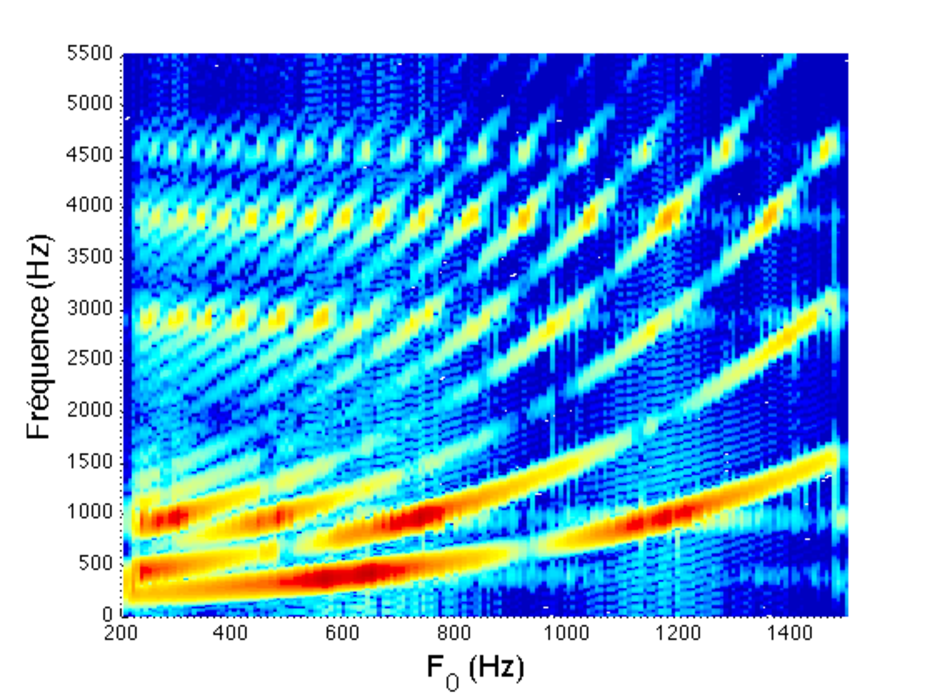
\includegraphics[width=.45\linewidth]{ch2/fig/Fi-F0-dpdce-sans_soprano_u_200-1500Hz_dig13b3.pdf}}
%   \label{Fig:Fi-F0-dpdce_sans}
%   \hspace{0.3cm}
%   \subfloat
% 	[{\it Avec dépendances}]  
%   {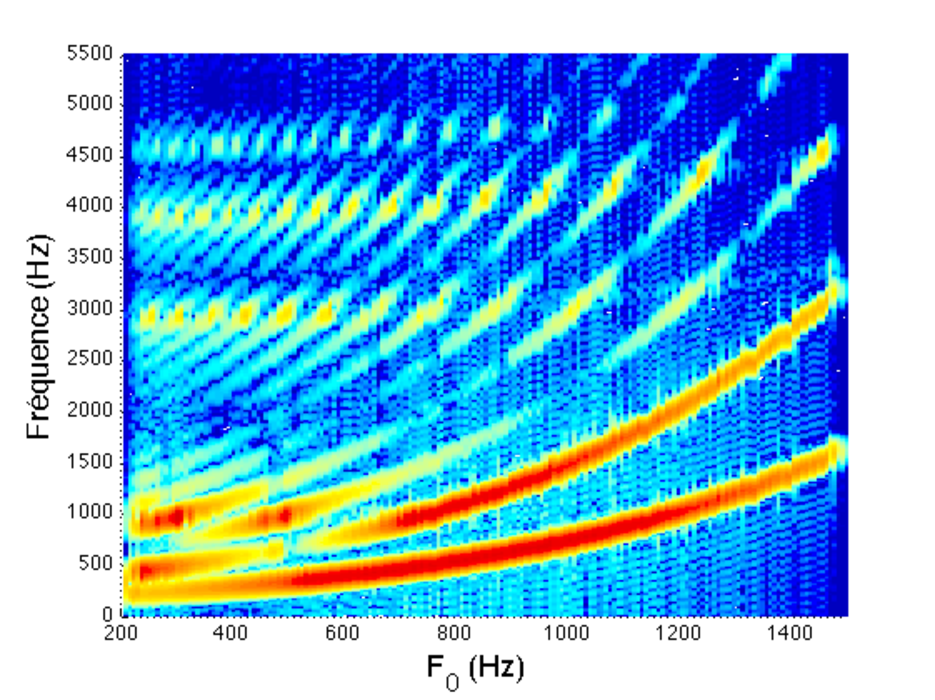
\includegraphics[width=.45\linewidth]{ch2/fig/Fi-F0-dpdce-avec_soprano_u_200-1500Hz_dig13b3.pdf}}
%   \label{Fig:Fi-F0-dpdce_avec}
%     \caption{{\it Spectrogrammes de la voyelle /a/ de synthèse, où $F_0$ augmente avec le temps, (a) sans ou (b) avec les dépendances entre les fréquences centrales des formants et de $F_0$. \textit{Voir fichiers audios~/ vidéos~\ref{fav:fi-f0-dependance}}\\
% }}
%   \label{Fig:Fi-F0-dpdce}
% \end{figure}

% \subsubsection{a) La soufflerie}

% \begin{table}[!h]
% 	\centering
% 	\begin{tabular}{|c|c|c|} 
% 		\hline
% 		& \centering \textbf{Tessiture naturelle moyenne} & \centering \textbf{Tessiture
% dans le synthétiseur} \tabularnewline
% 		\hline
% 		\bf Basse & Mi2-Mi4 & Sol$\sharp$1-Sol4\\
% 		\hline
% 		\bf Ténor & Do3-Si4 & Sol$\sharp$1-Sol4\\
% 		\hline
% 		\bf Alto & Fa3-Mi5 & Sol$\sharp$2-Sol5\\
% 		\hline
% 		\bf Soprano & Si3-Do6 & Sol$\sharp$3-Sol6\\
% 		\hline
% 	\end{tabular}
% 	\caption{\textit{Tessiture des chanteurs naturels et synthétiques (La3=440 Hz). Voir fichiers audios~/ vidéos~\ref{fav:types-voix-1}}}
% 	\label{Tab:tessChant}
% \end{table}

